
In this section we study the uncertainties on the shape of the MVA output for  
$H \to WW$ signal events. The signal prediction is generated using the POWHEG 
Monte Carlo generator, where the Higgs $p_{T}$ spectrum has been reweighted 
to the one predicted by the HQT program, which computes the resummed differential
cross section for the Higgs $p_{T}$ at next-to-next-to-leading order. We study
the uncertainties on the shape of the MVA output from the two primary 
sources of uncertainty: higher order corrections and parton distribution
function uncertainties.

First to obtain some intuition about the particular phase space that the
MVA is preferentially selecting, we compare the distributions of the 
MVA input observables for the signal sample with no selection requirements
and the signal sample where the MVA predict a high score for the signal.
The comparisons are shown in Figure \ref{fig:MVAHighScorePhaseSpaceRegion}
for the six MVA input observables where a cut of the MVA output greater 
than $0.8$ has been made for the MVA trained with the $M_{H} = 130$ GeV
signal hypothesis. We observe that the MVA selects the region of
low $\Delta\phi$, low $\Delta$R, low dilepton mass, and transverse 
mass closer to the higgs mass hypothesis. 

%%%%%%%%%%%%%%%%%%%%%%%%%%%%%%%%%%%
\begin{figure}[!htbp]
\begin{center}
\subfigure[PtMax]{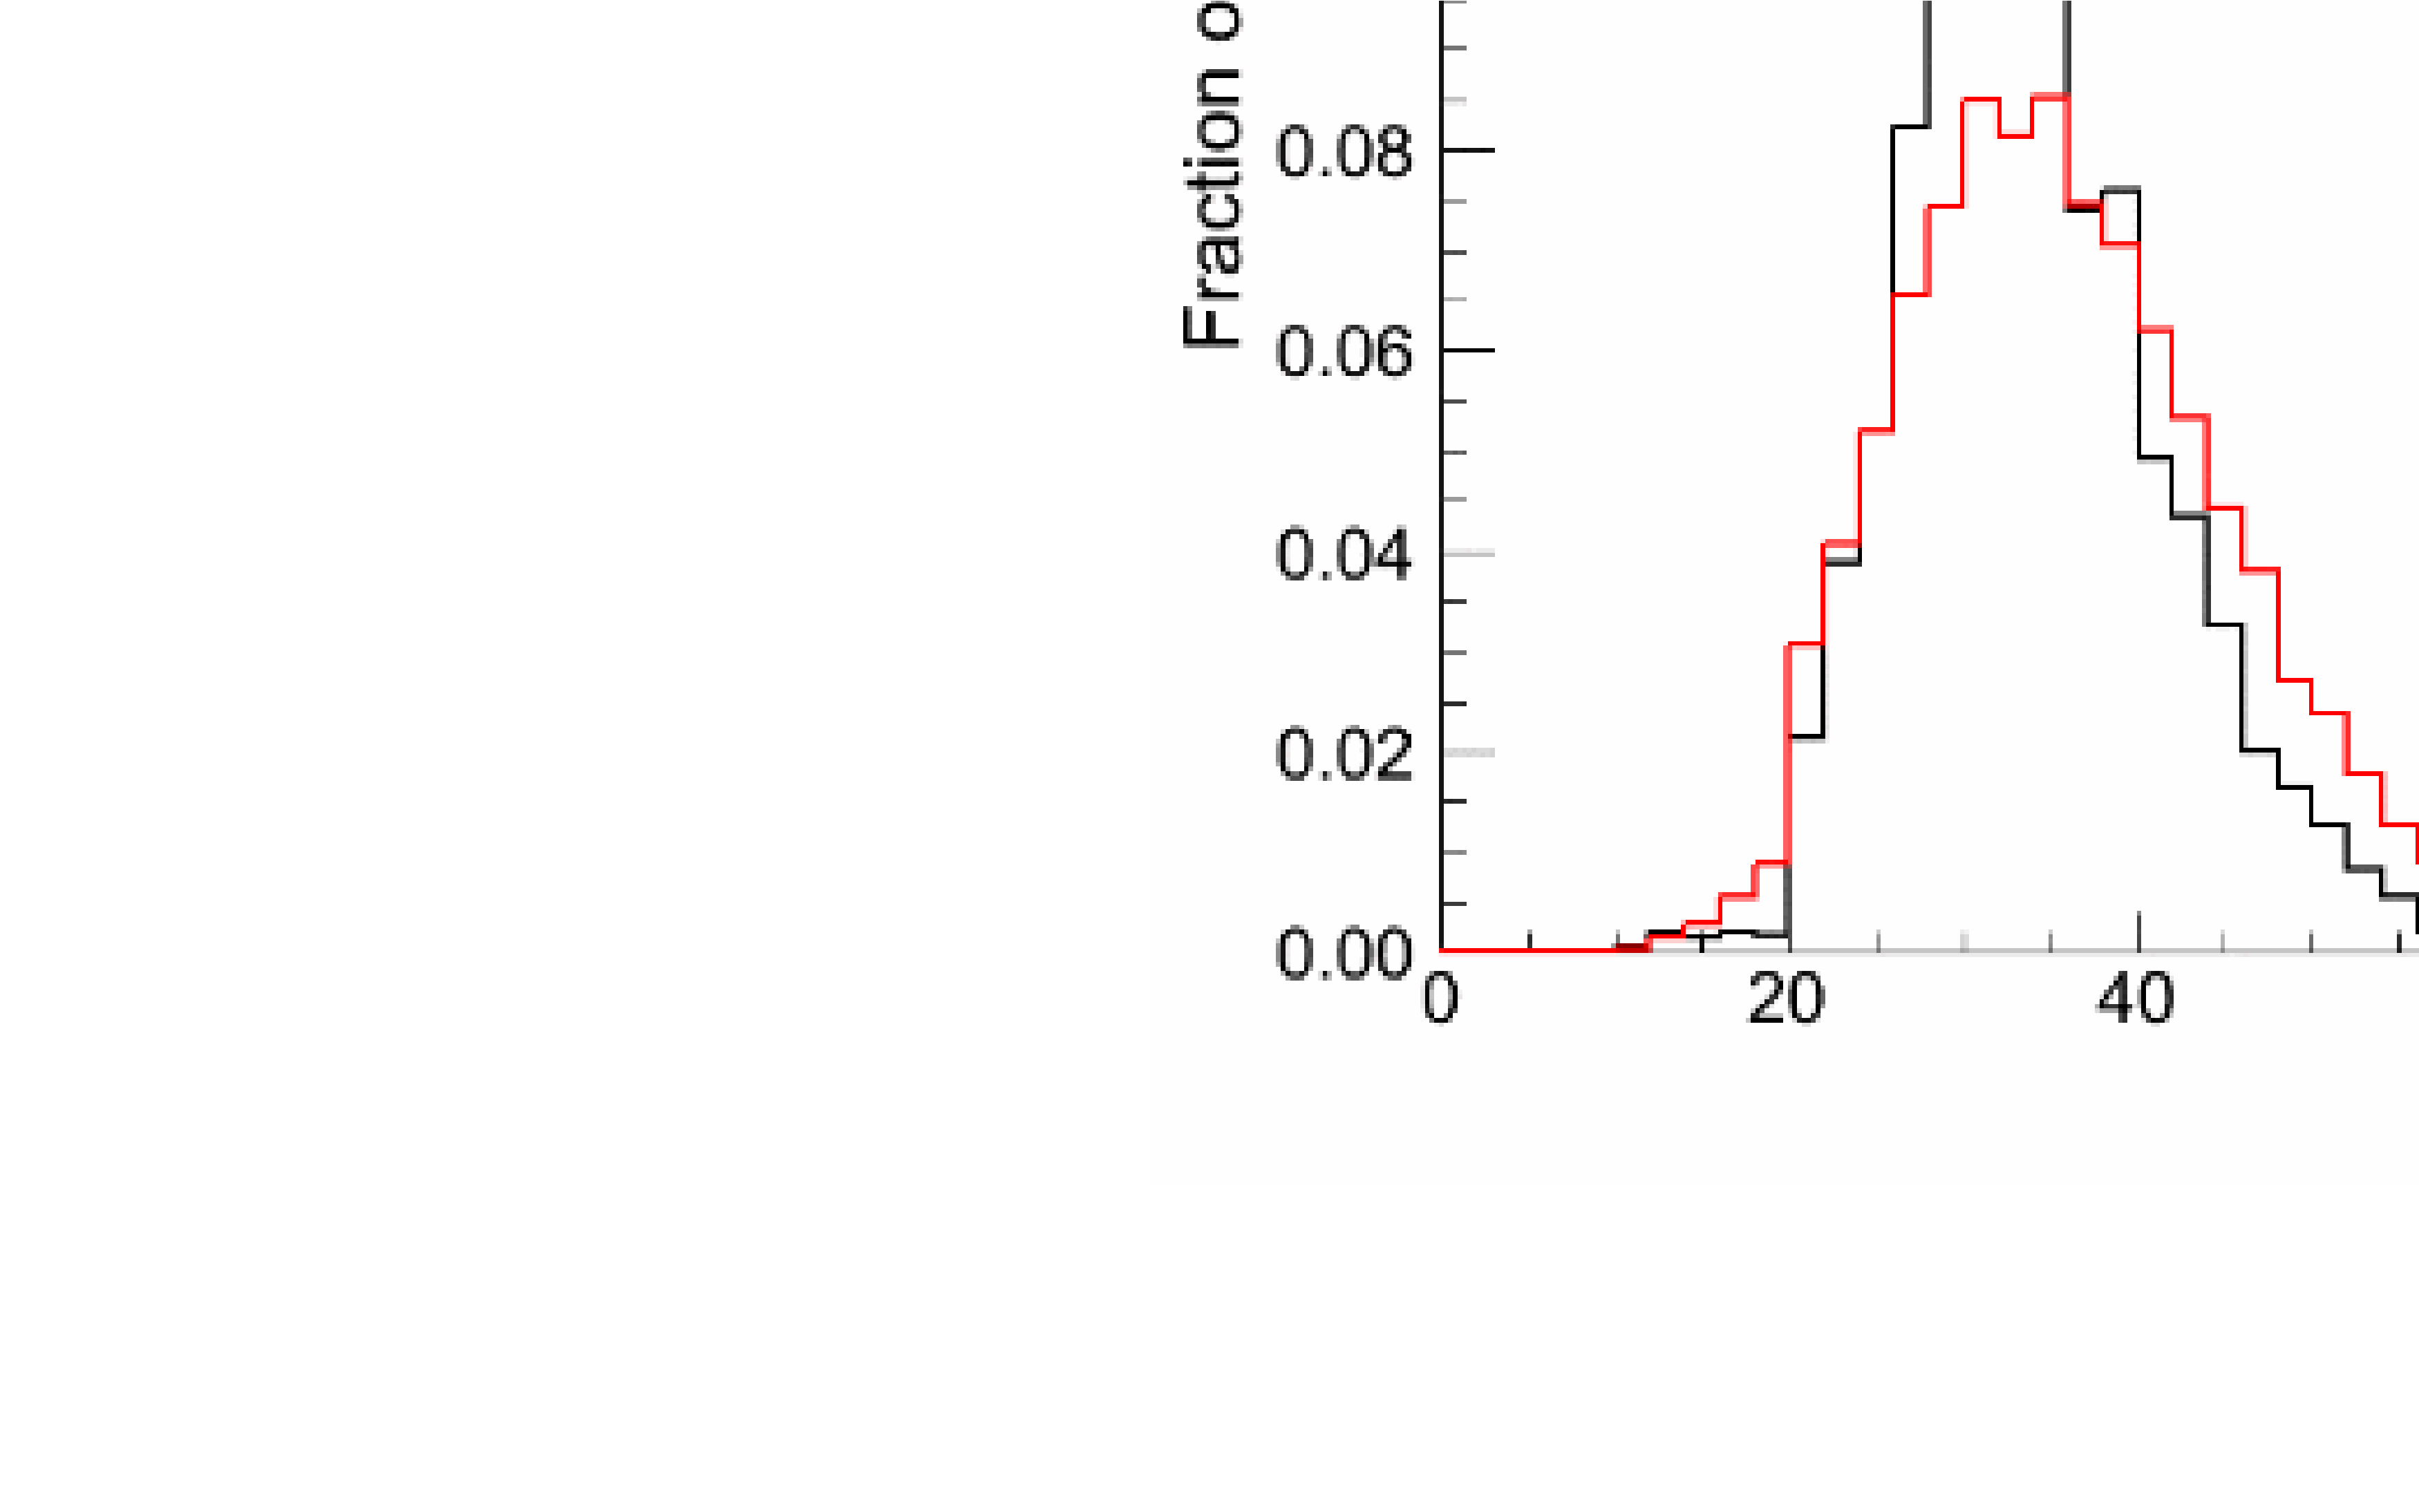
\includegraphics[width=0.49\textwidth]{figures/MVAHighScorePhaseSpace_MVA130_PtMax.pdf}}
\subfigure[PtMin]{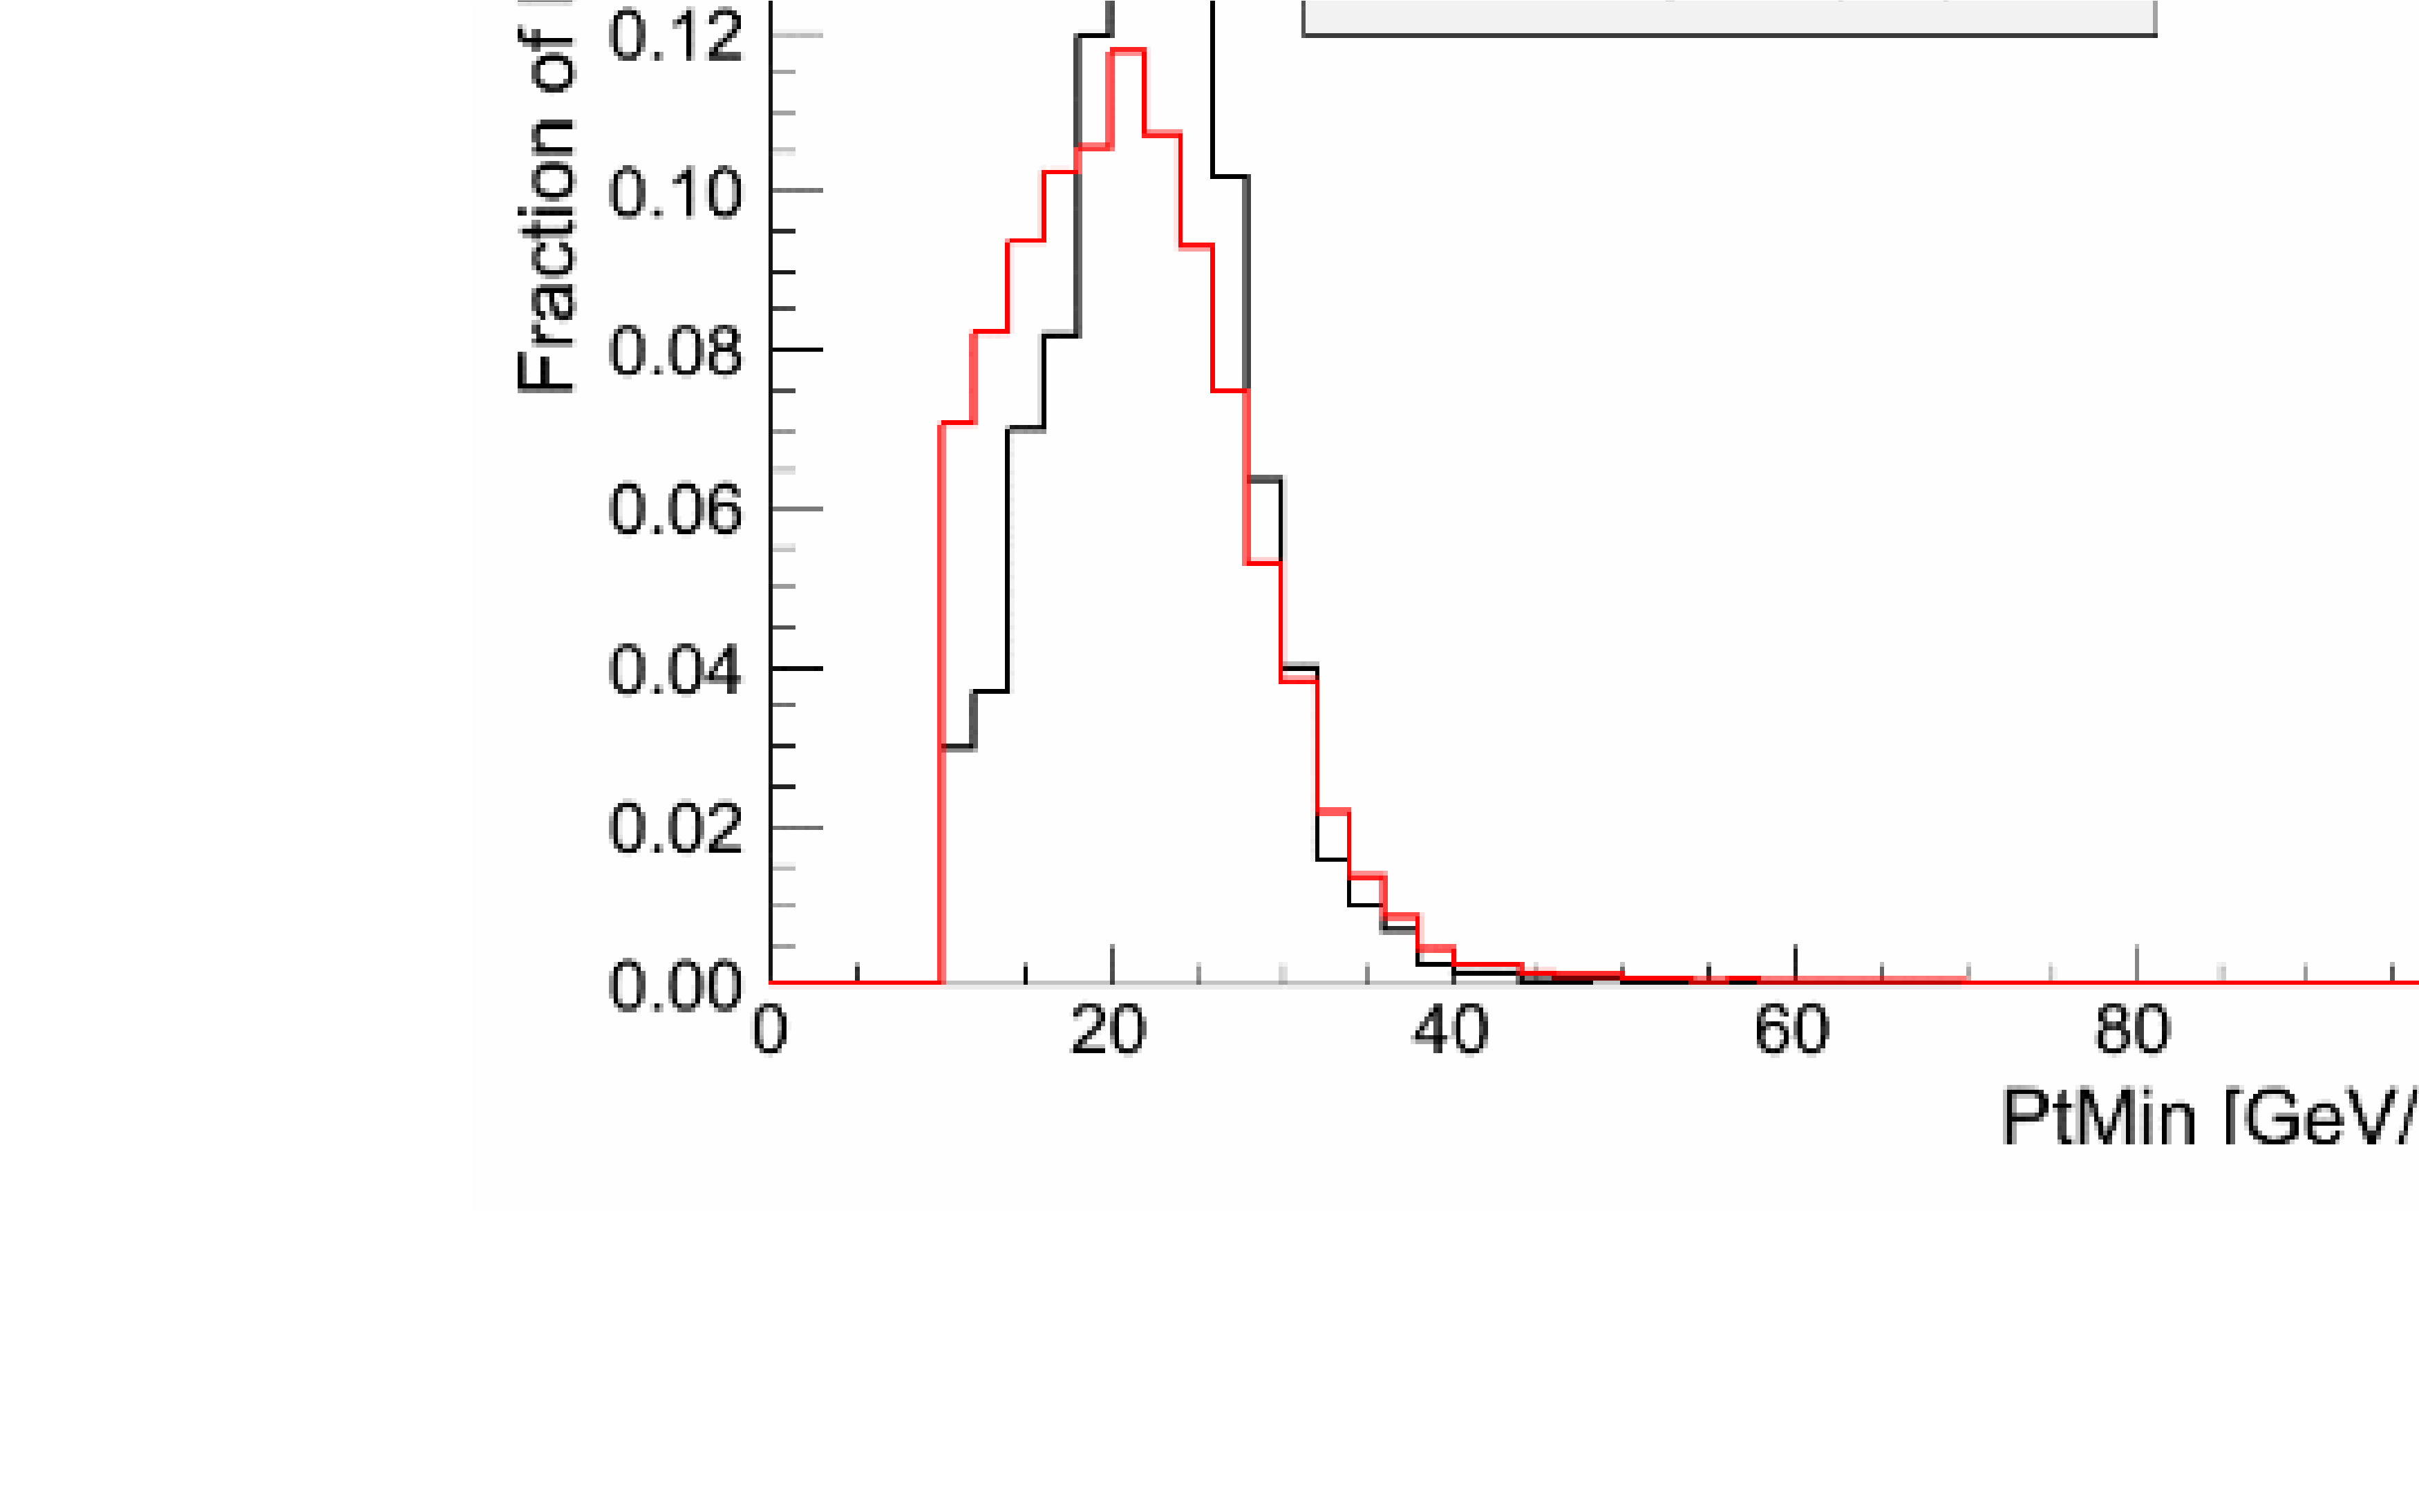
\includegraphics[width=0.49\textwidth]{figures/MVAHighScorePhaseSpace_MVA130_PtMin.pdf}}  
\\
\subfigure[$M_{\mathrm{ll}}$]{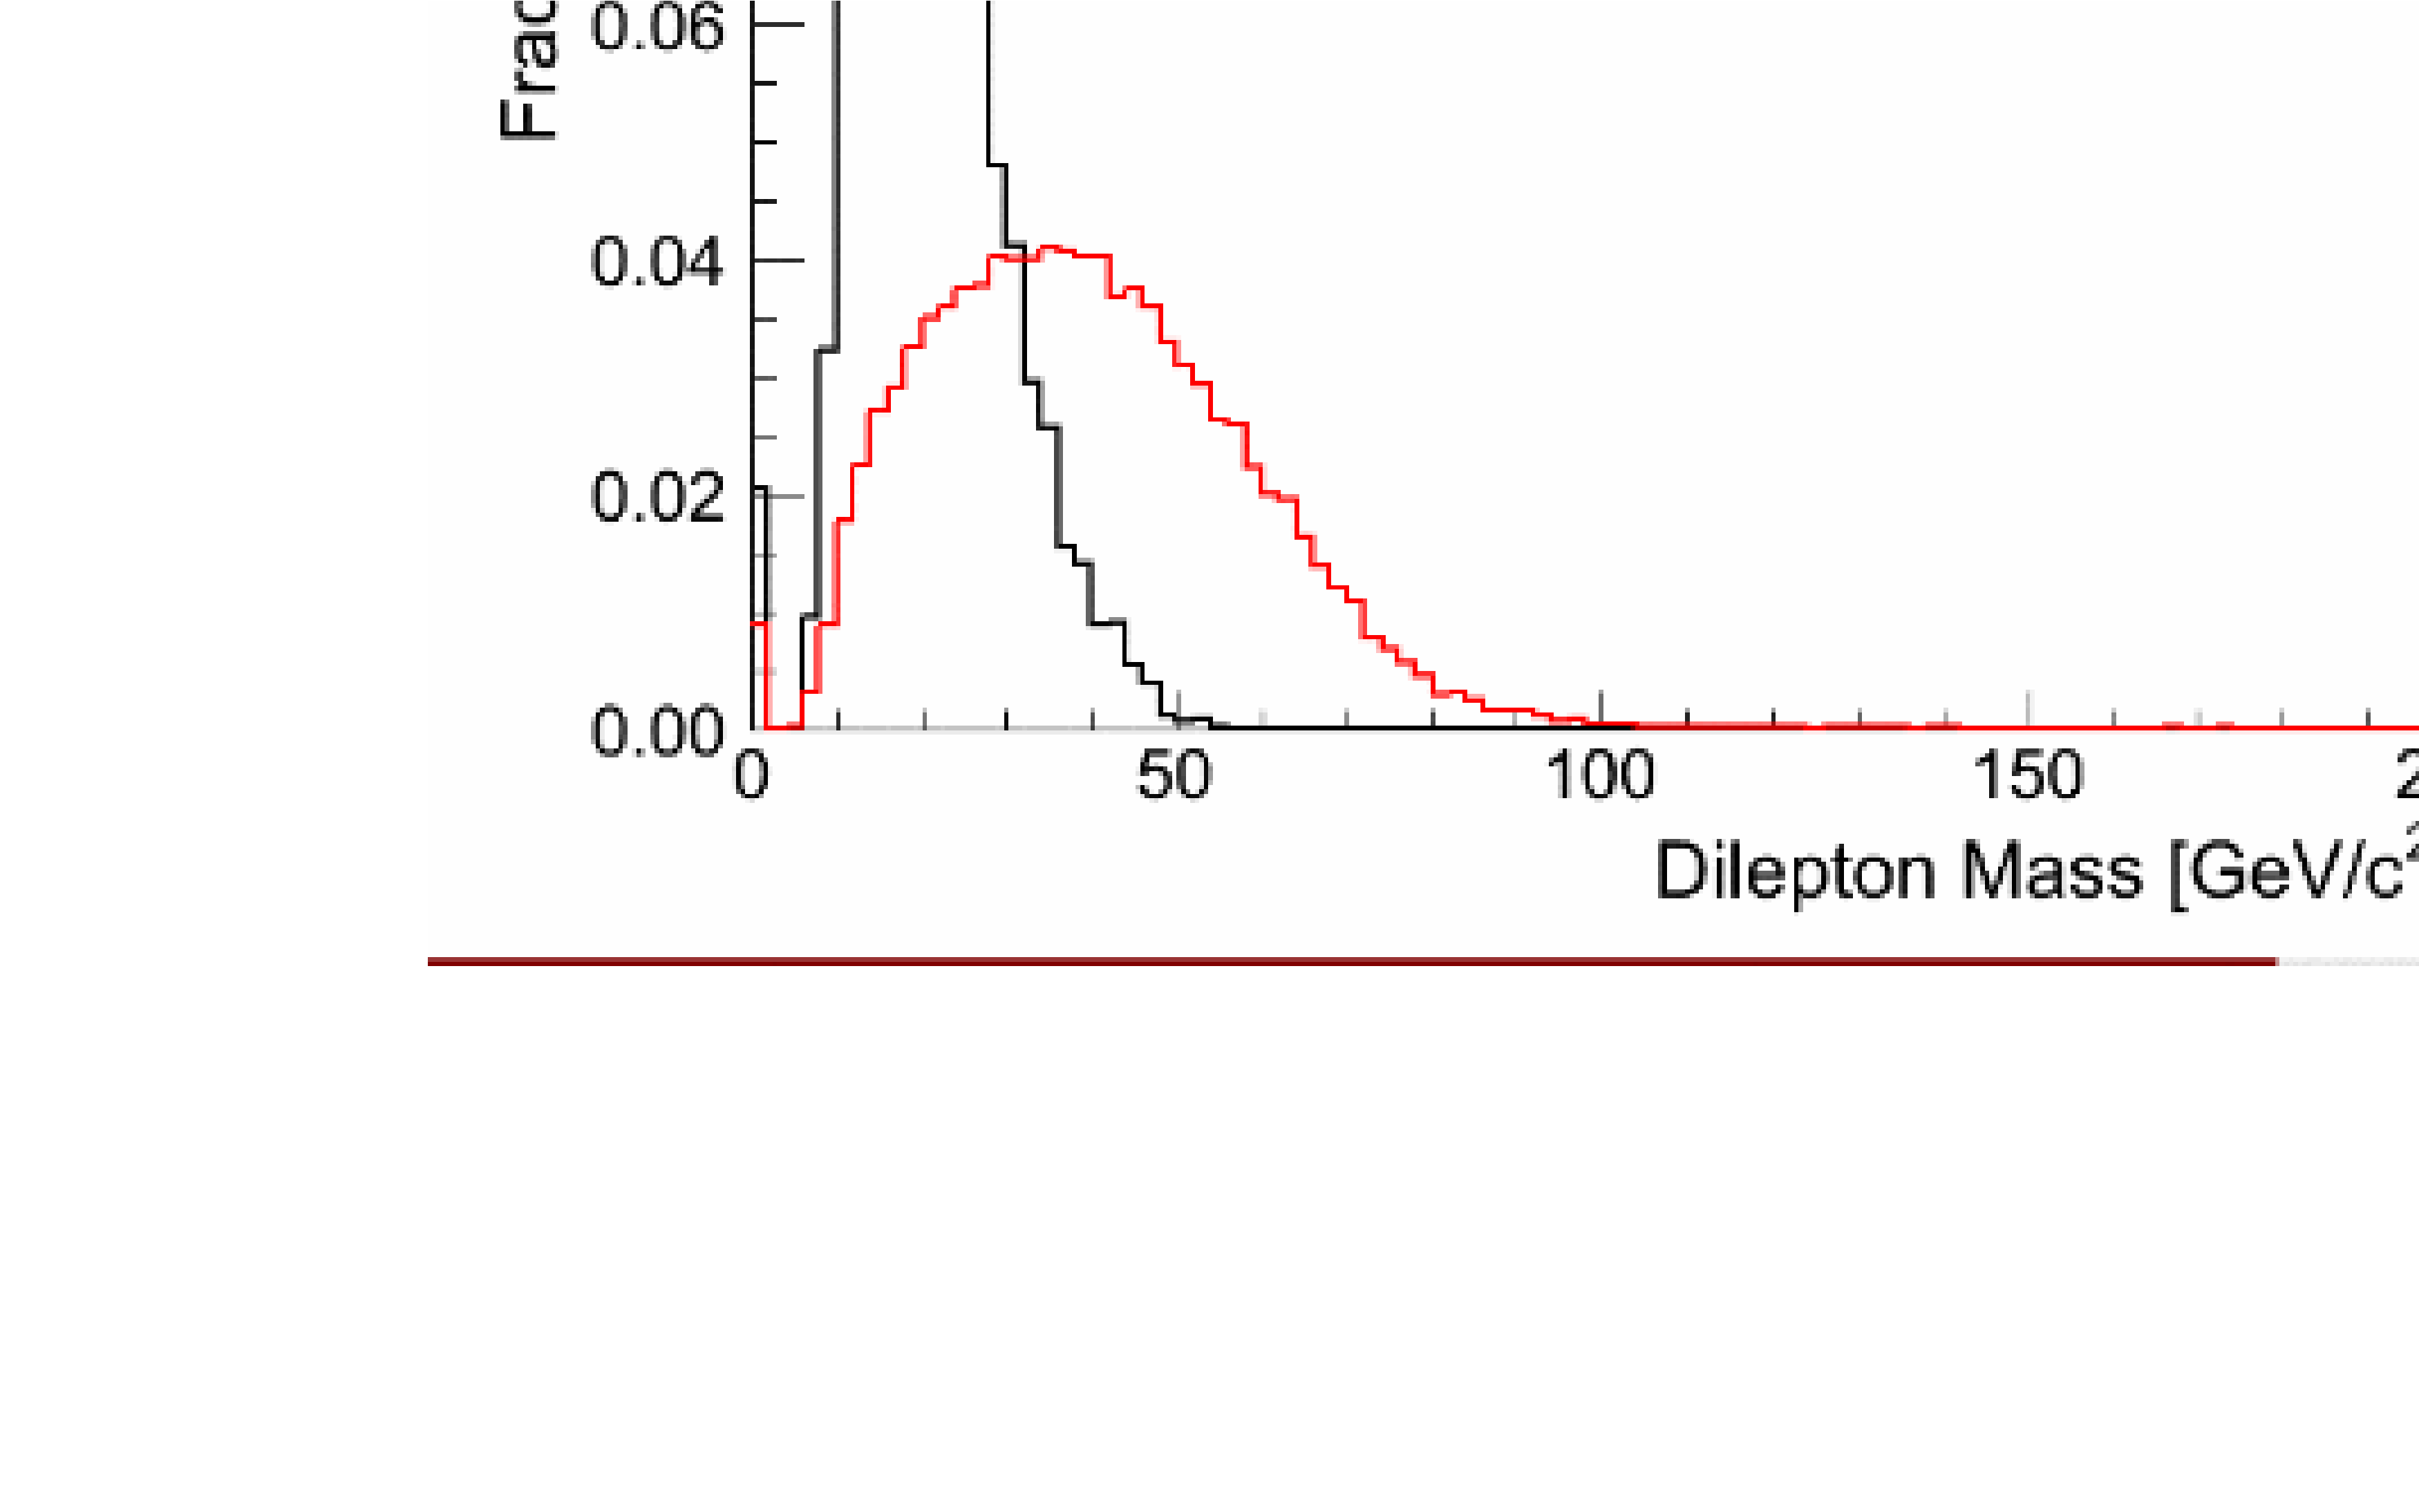
\includegraphics[width=0.49\textwidth]{figures/MVAHighScorePhaseSpace_MVA130_DileptonMass.pdf}}
\subfigure[$M_{\mathrm{T Higgs}}$]{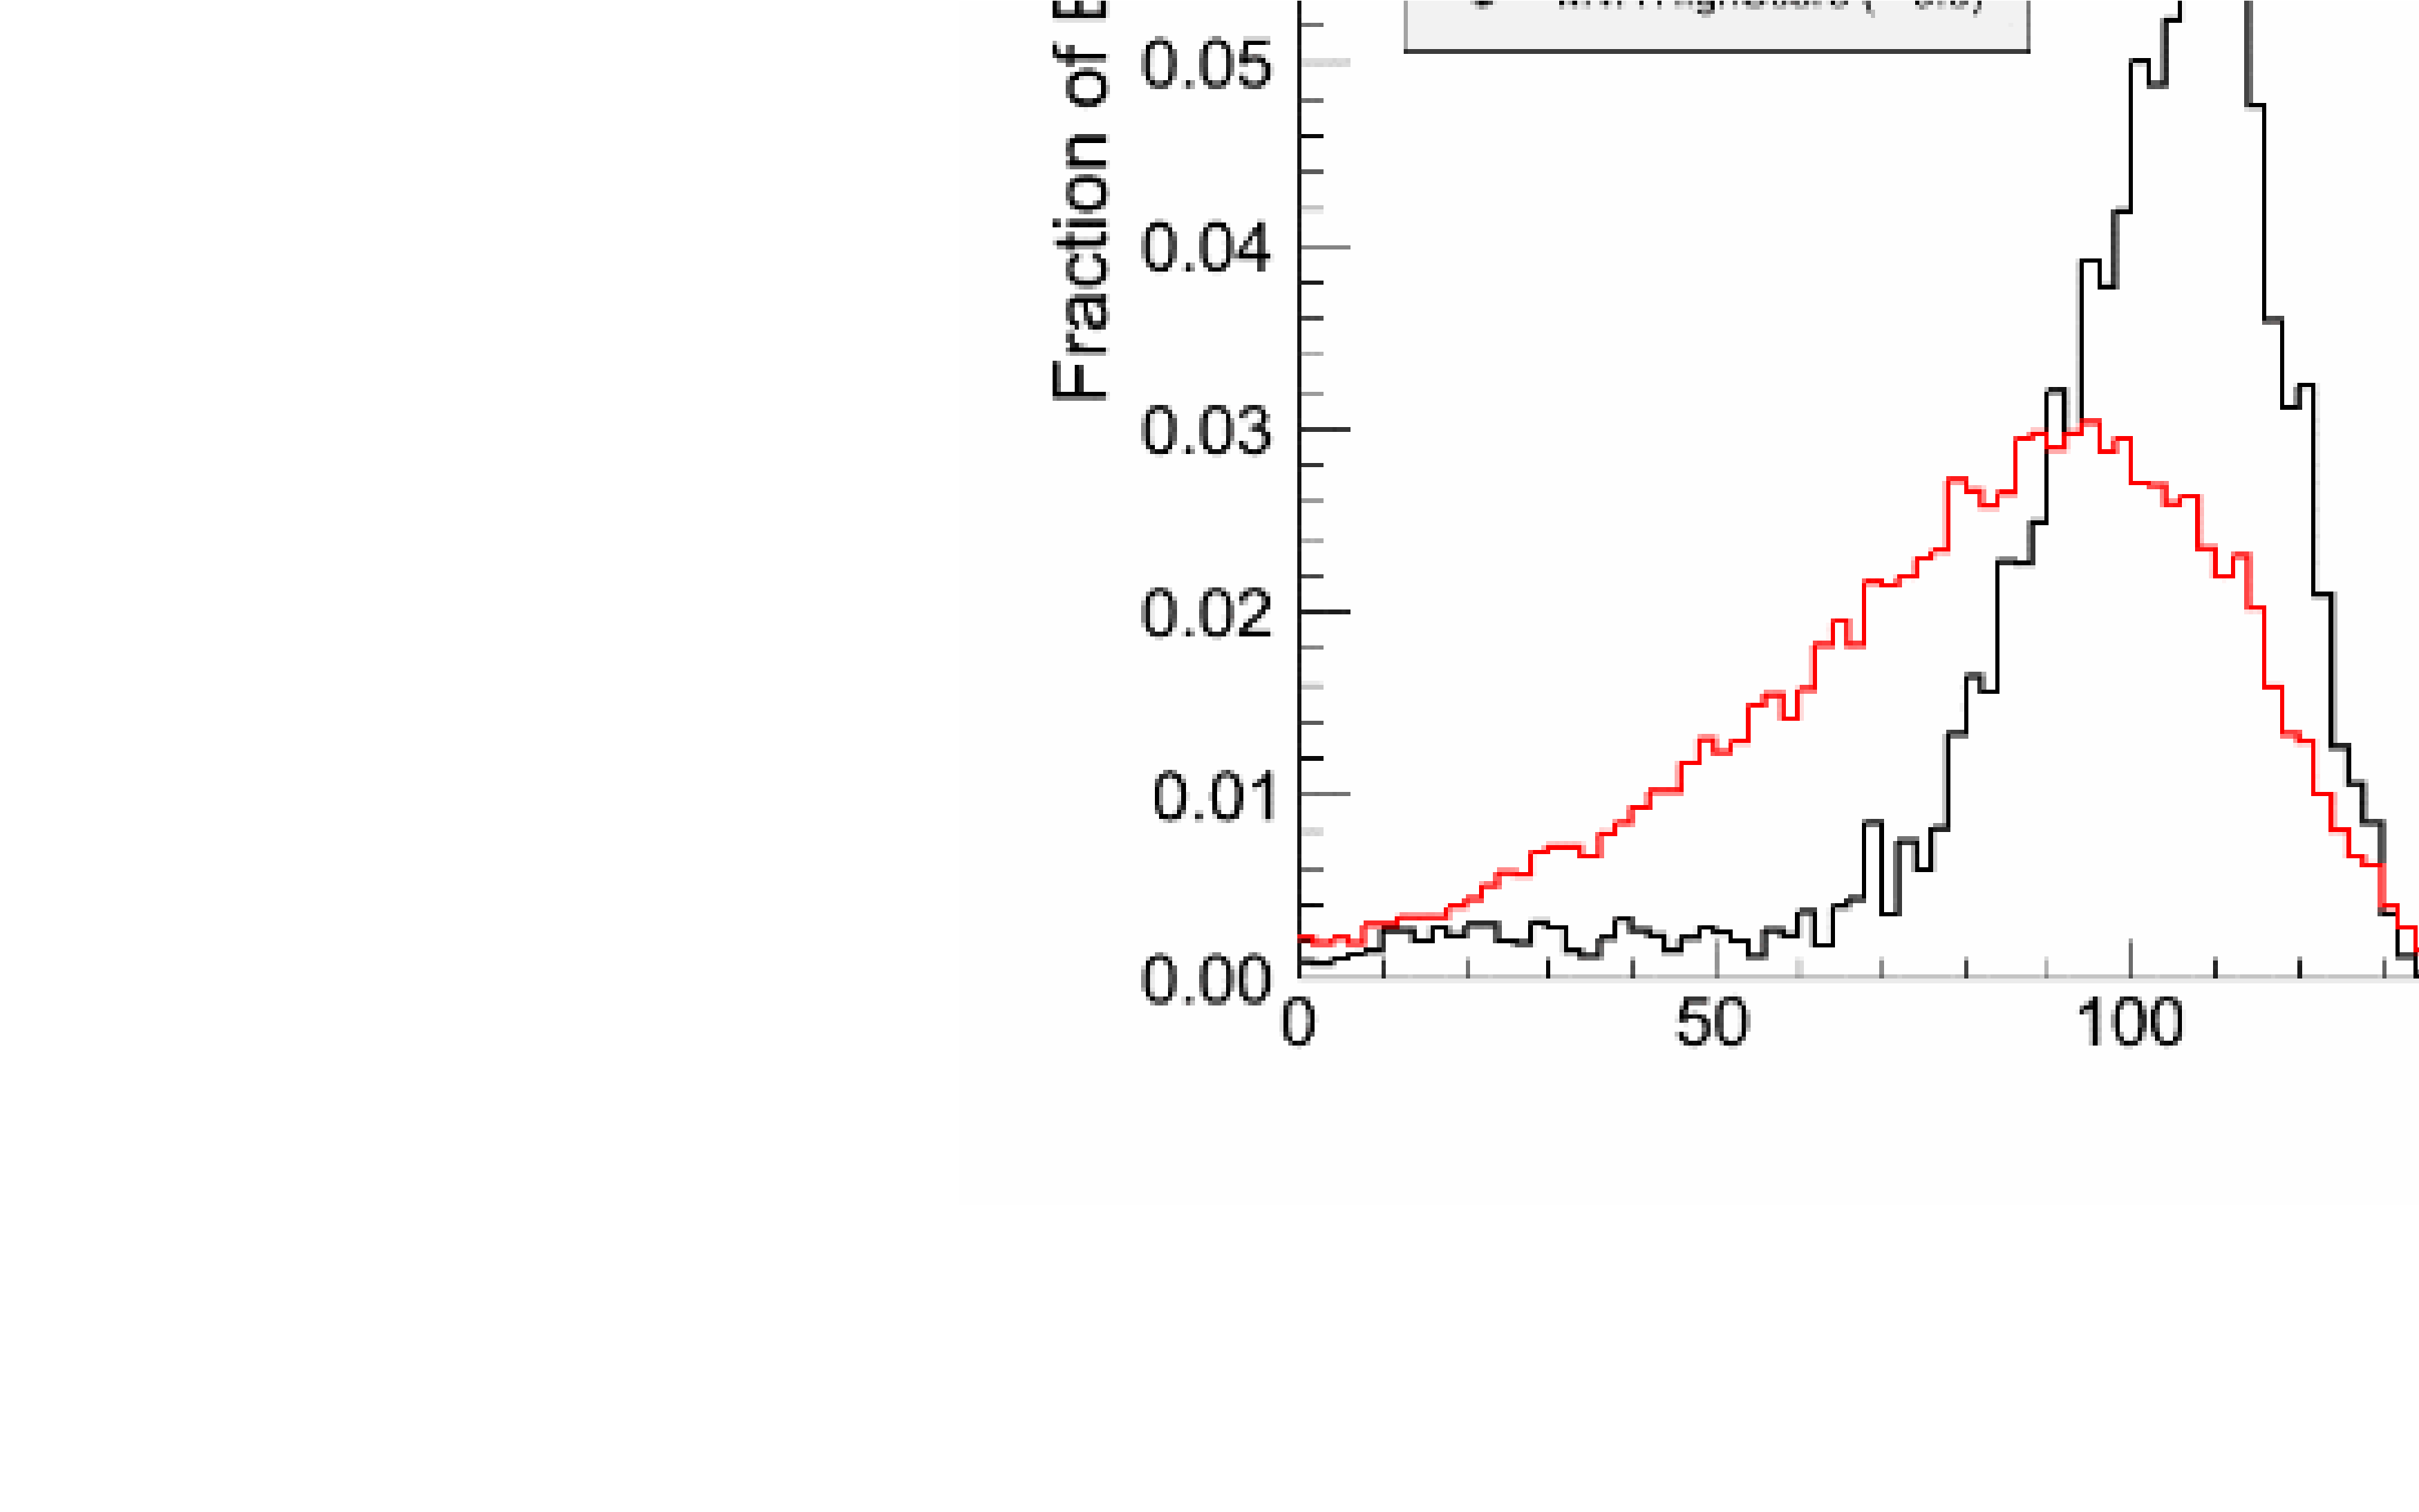
\includegraphics[width=0.49\textwidth]{figures/MVAHighScorePhaseSpace_MVA130_MTHiggs.pdf}}  
\\
\subfigure[$\Delta\phi_{\mathrm{ll}}$]{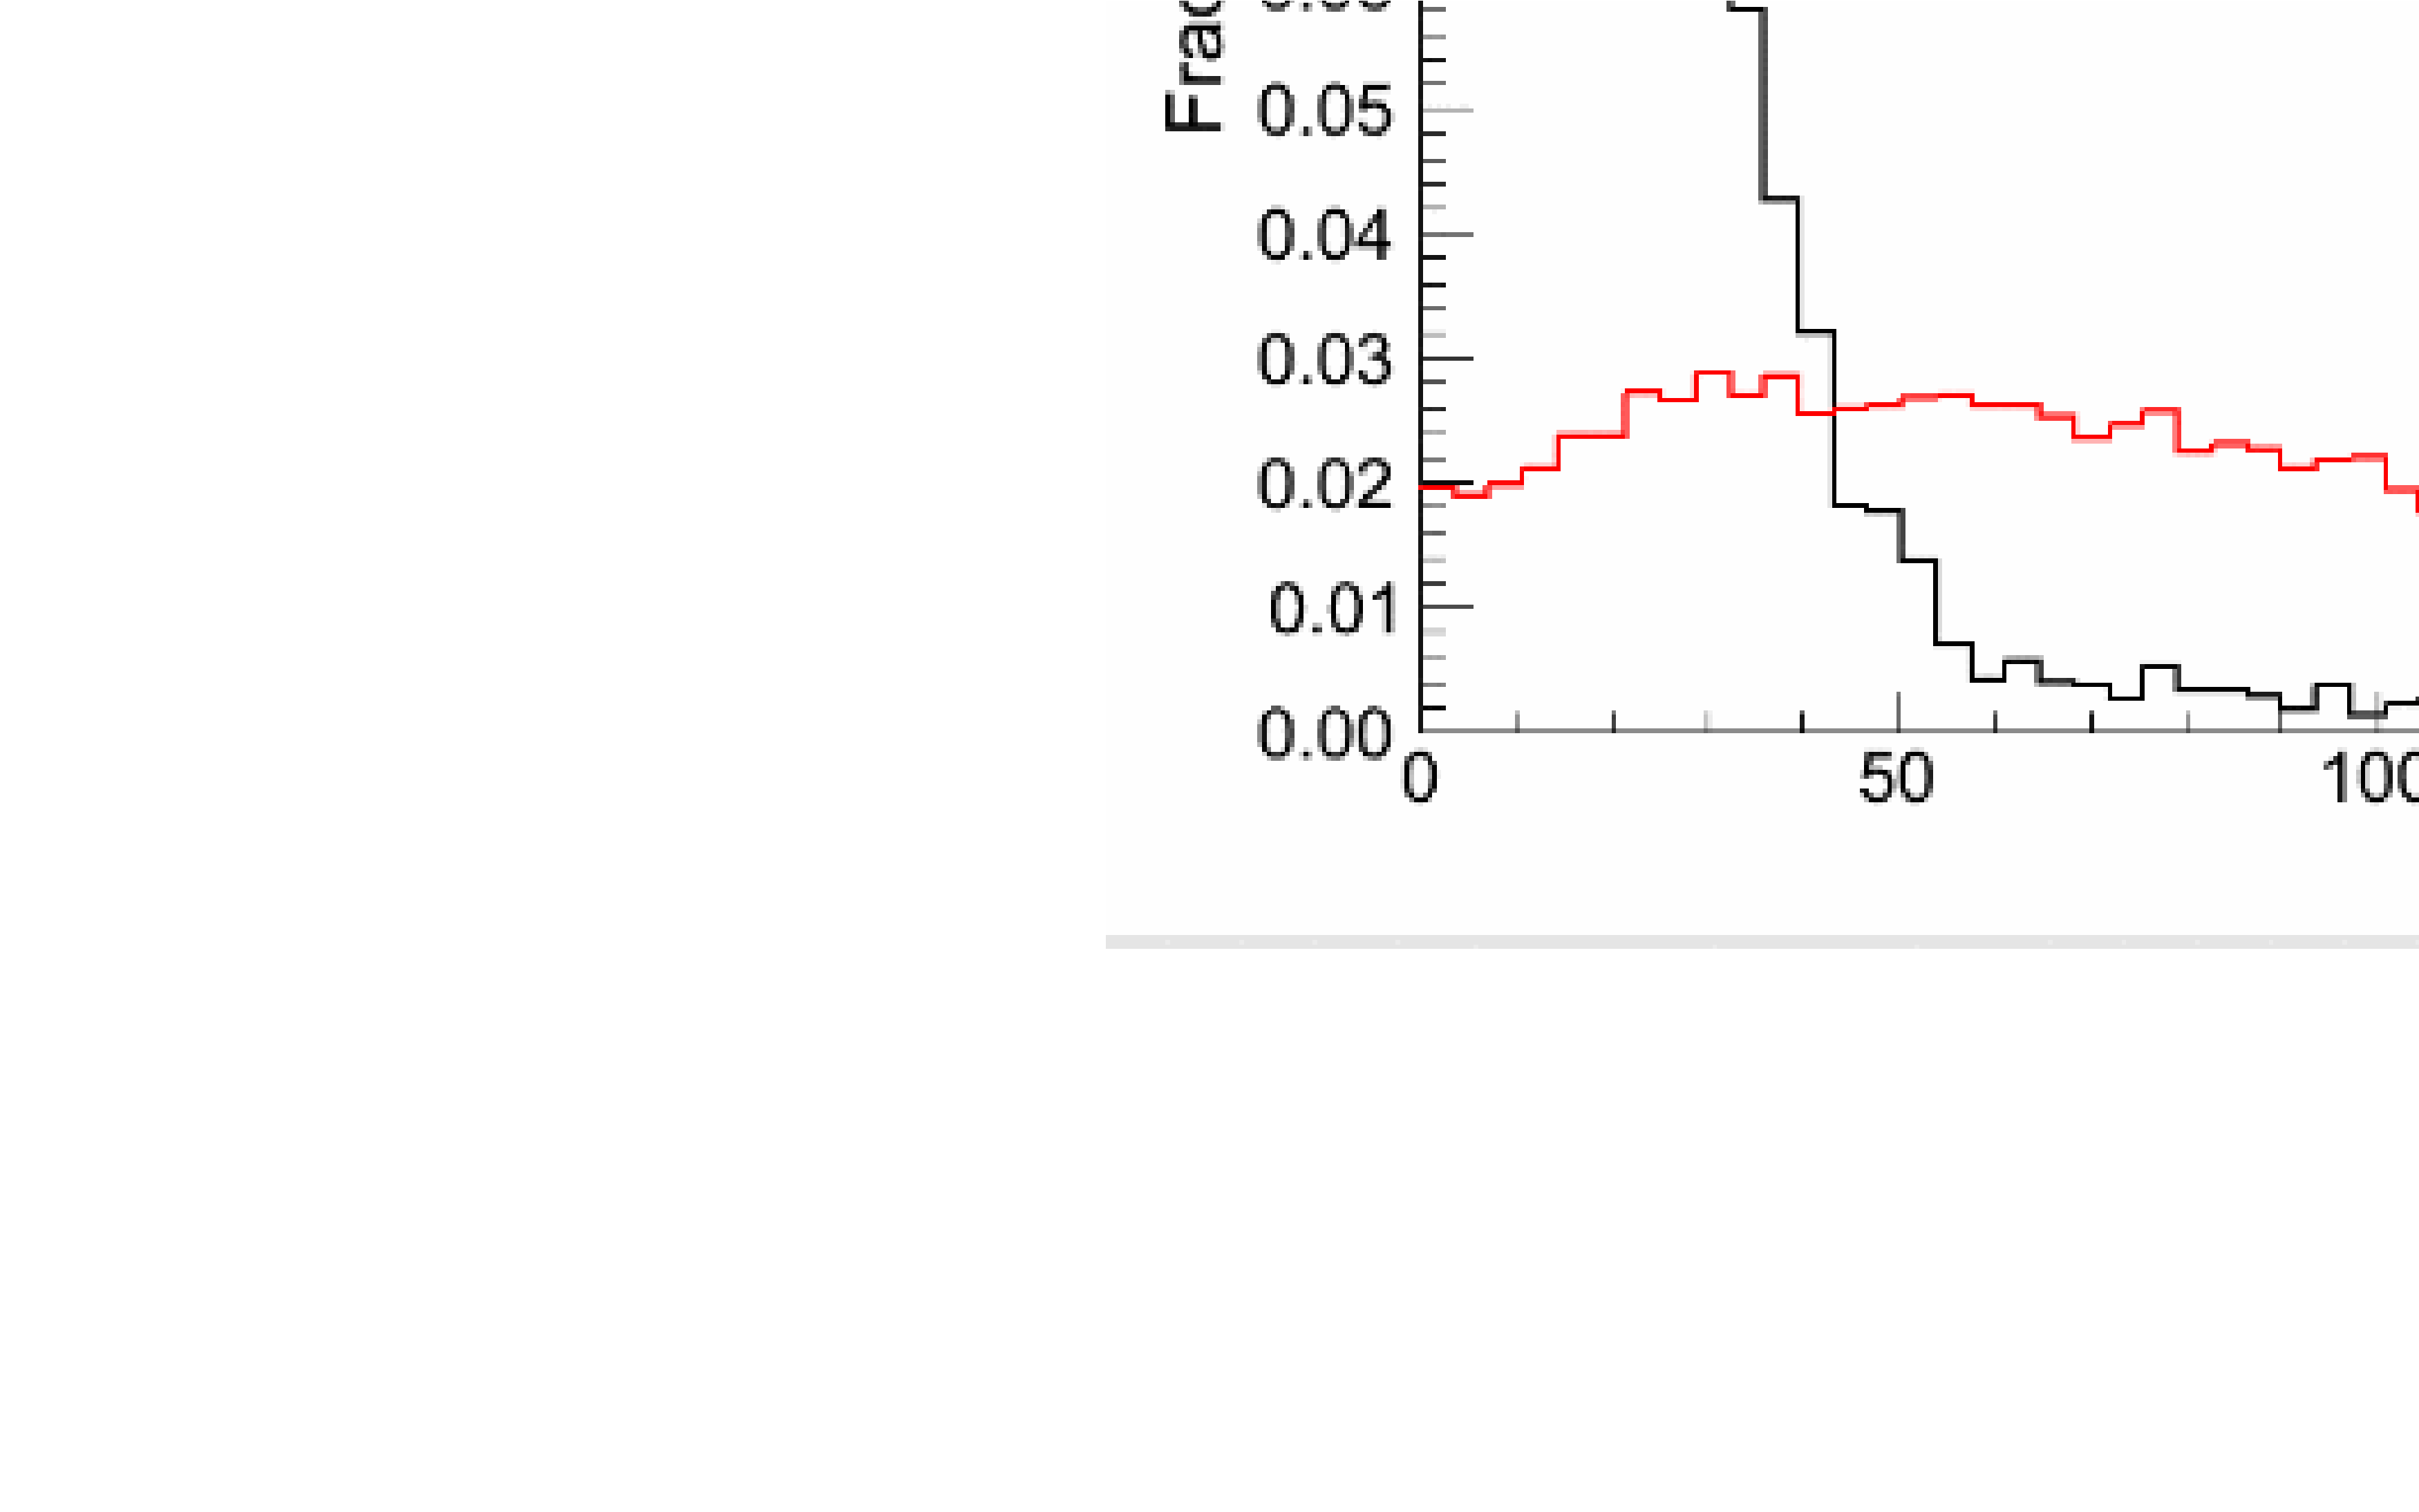
\includegraphics[width=0.49\textwidth]{figures/MVAHighScorePhaseSpace_MVA130_DeltaPhi.pdf}}
\subfigure[$\Delta\mathrm{R}_{\mathrm{ll}}$]{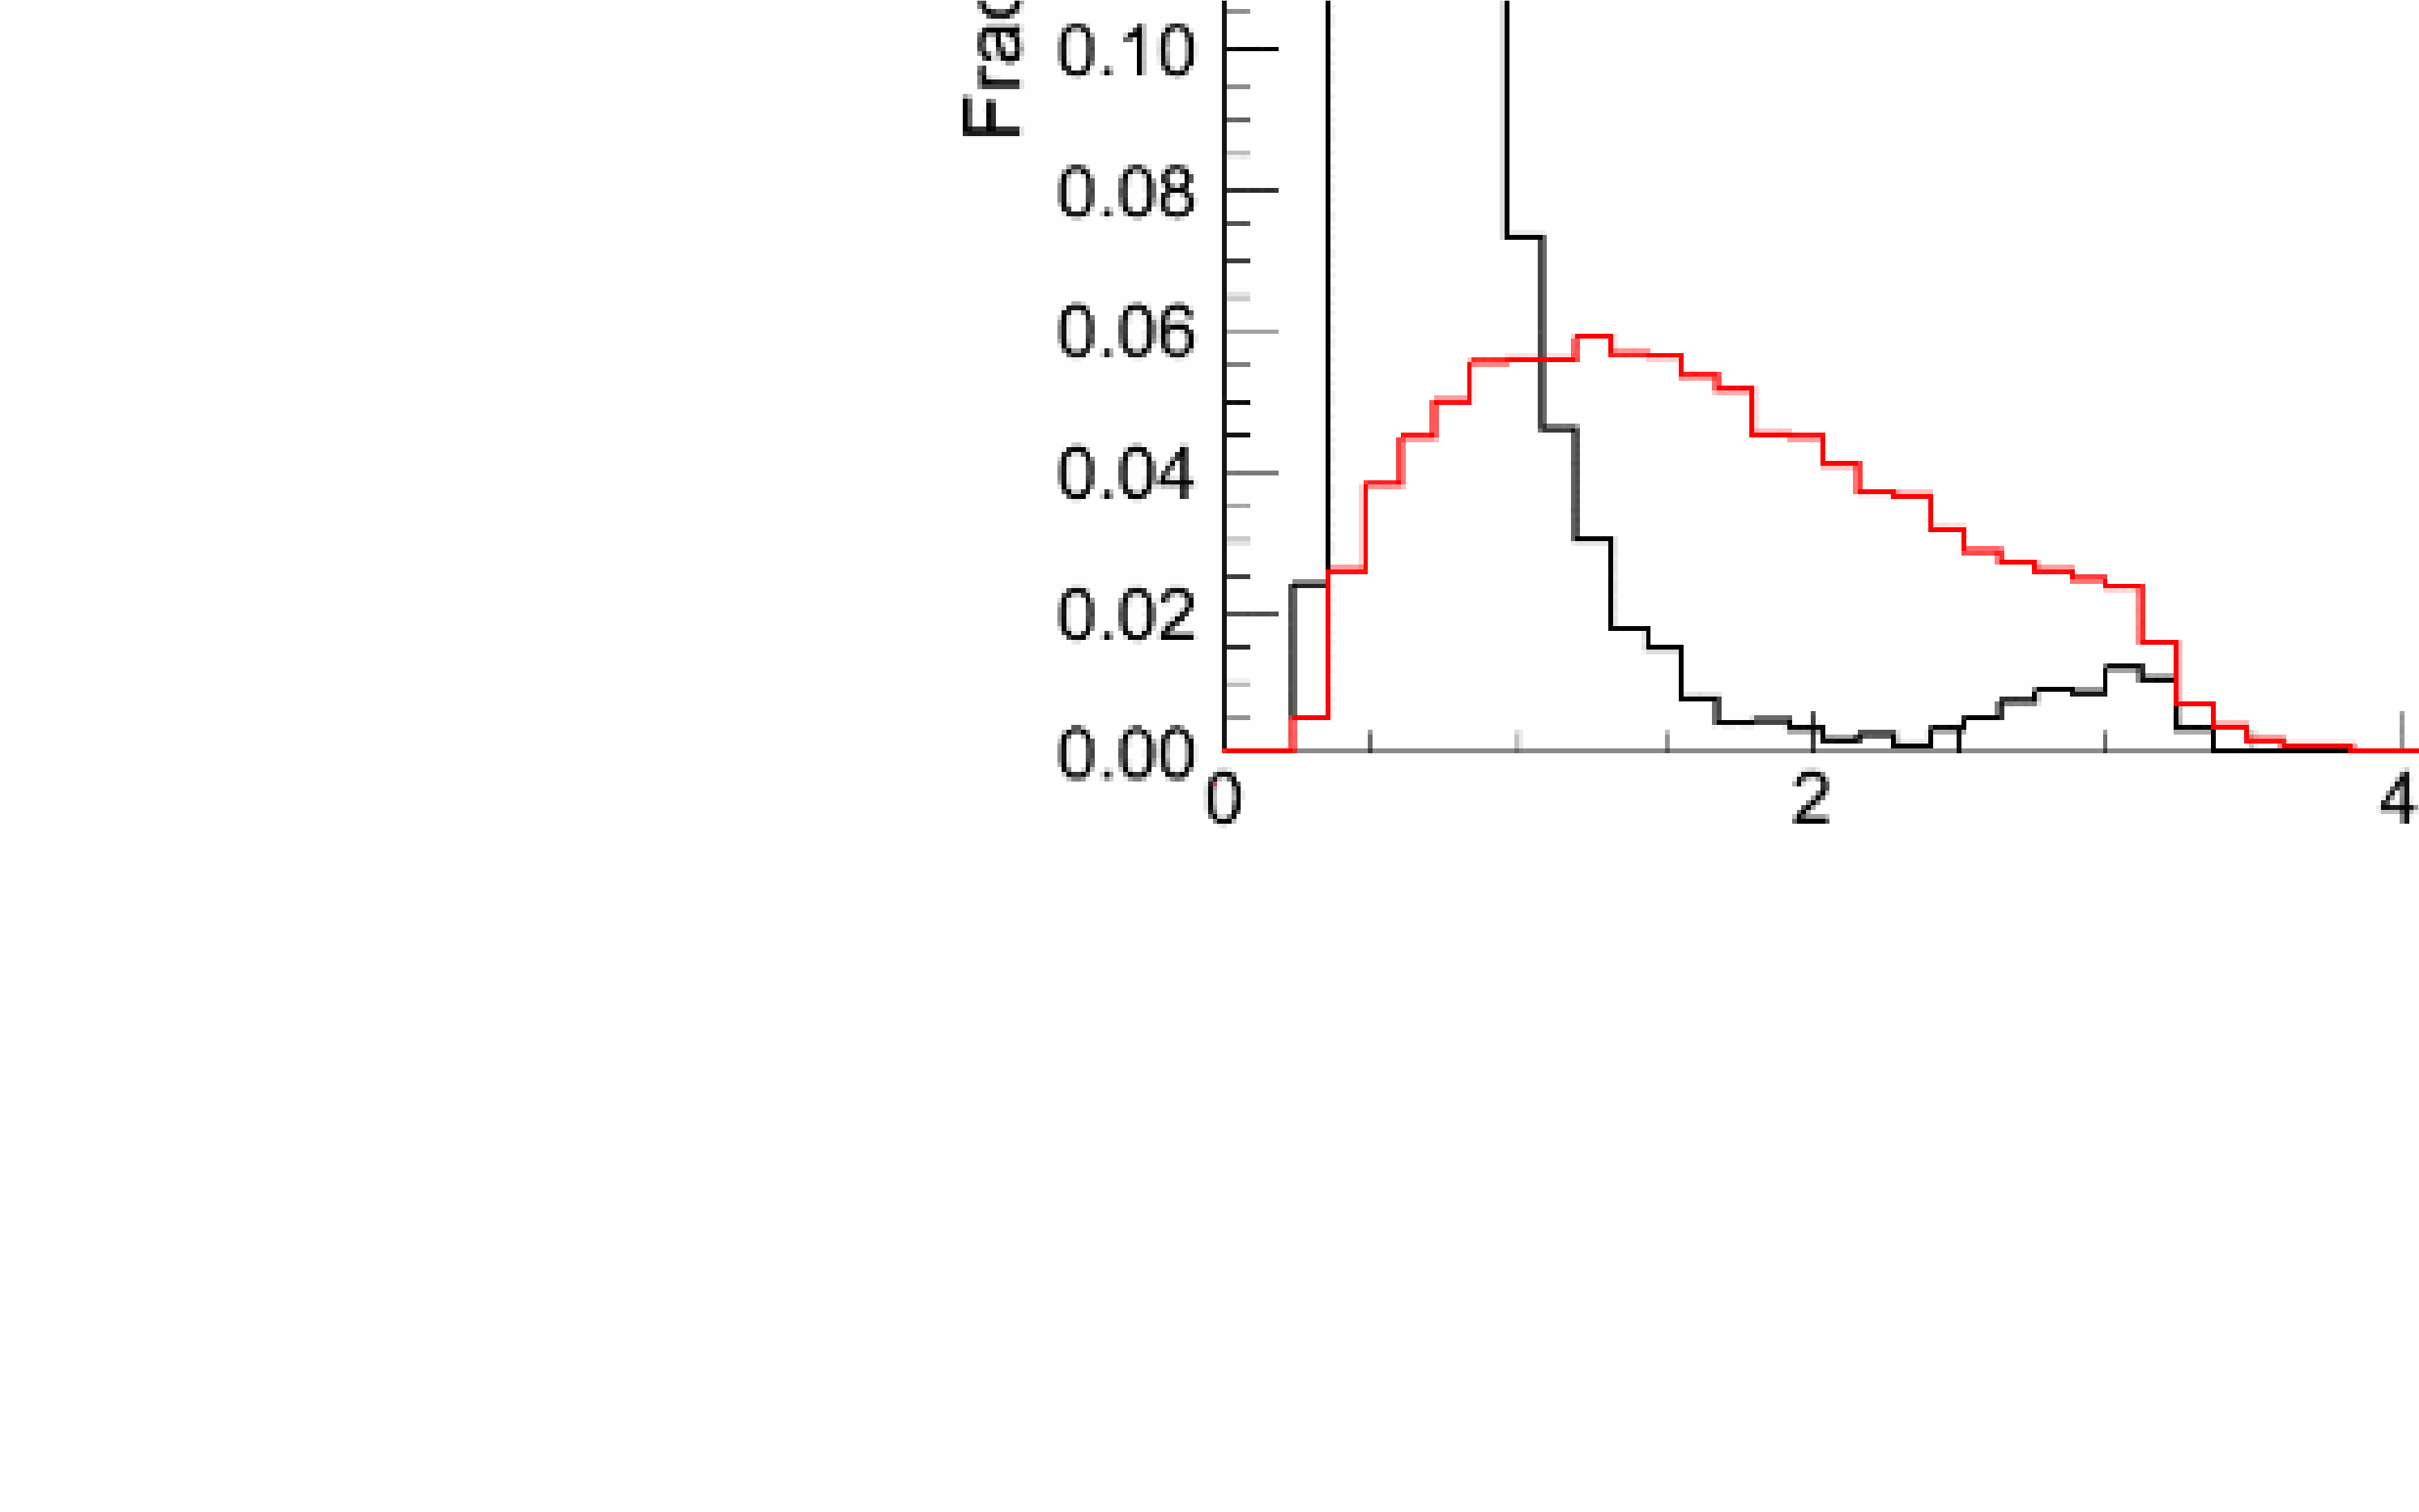
\includegraphics[width=0.49\textwidth]{figures/MVAHighScorePhaseSpace_MVA130_DeltaR.pdf}}
\caption{Comparisons of the distribution of the MVA input observables for the
inclusive sample of signal events and the sample of signal events where a
high score of the MVA is required (MVA $>0.8$).
}
\label{fig:MVAHighScorePhaseSpaceRegion}
\end{center}
\end{figure}
%%%%%%%%%%%%%%%%%%%%%%%%%%%%%%%%%%%


\subsubsection{Higher Order Corrections}

We factorize the effect of the higher order corrections into two
pieces: the effect of higher order corrections on the Higgs $p_{T}$ spectrum
and the effect of higher order corrections on everything else. To study the
effect on the Higgs $p_{T}$ spectrum we produce $p_{T}$ spectra using HQT
with the renormalization and factorization scales varied up and down by factors 
of $2$ and $1/2$, shown in Figure \ref{fig:signalshape_PtSpectrumScaleVariation_HiggsPt}.

%%%%%%%%%%%%%%%%%%%%%%%%%%%%%%%%%%%
\begin{figure}[!htbp]
\begin{center}
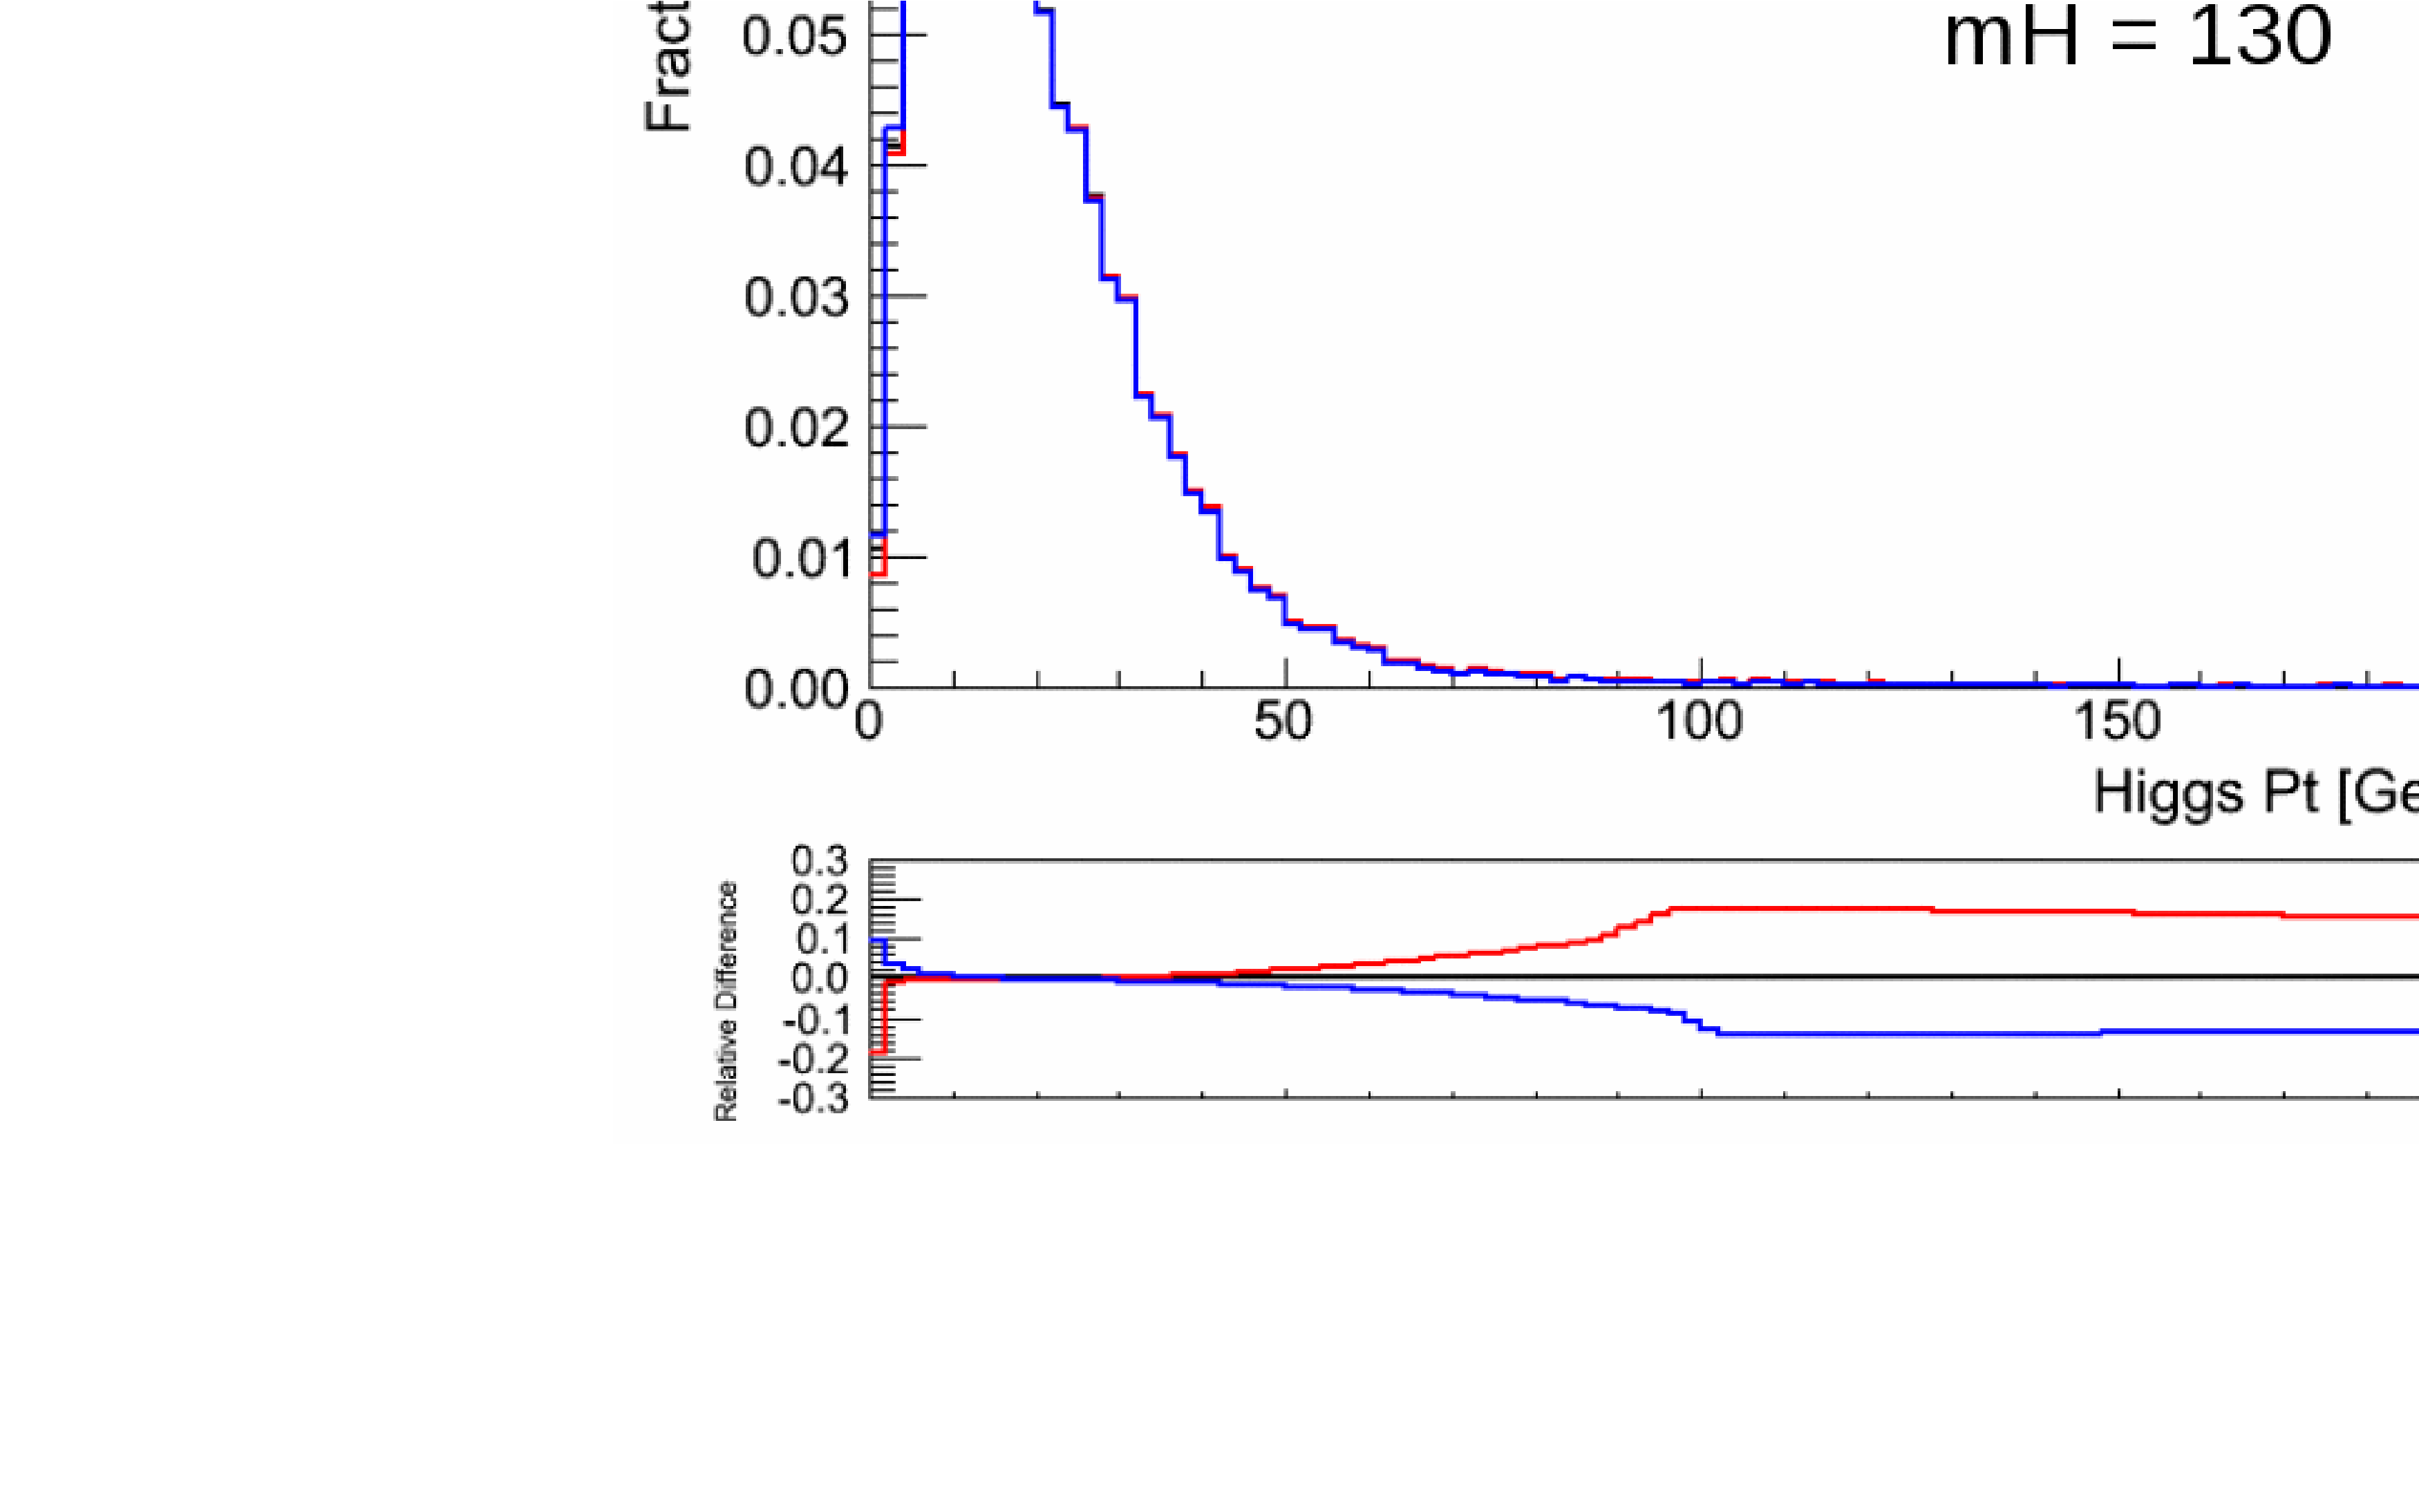
\includegraphics[width=0.49\textwidth]{figures/ShapeSystematics_HWW_HiggsPt_HQTScaleVariation.pdf}
\caption{Comparison of the resummed NNLO predicted Higgs $p_{T}$ spectrum with variations of
the renormalization and factorization scales.
}
\label{fig:signalshape_PtSpectrumScaleVariation_HiggsPt}
\end{center}
\end{figure}
%%%%%%%%%%%%%%%%%%%%%%%%%%%%%%%%%%%


These scale varied spectra give an indication of the
effect of the terms beyond NNLO in the perturbative expansion on the $p_{T}$ 
spectrum. Then we take the POWHEG Monte Carlo sample, reweight to the scale 
varied $p_{T}$ spectra, and compare the differences in the prediction of 
the distributions of the MVA input observables and the MVA output. In Figure
\ref{fig:signalshape_PtSpectrumScaleVariation_InputObservables} we show the
comparison for the four most important MVA input observables between the
Monte Carlo prediction reweighted to the scale varied $p_{T}$ spectra. We
observe that the effect of the scale variation is extremely small and only
visible as we approach the very high $p_{T}$ region of phase space. In Figure
\ref{fig:signalshape_PtSpectrumScaleVariation_MVAOutput} we show the comparison
of the MVA output distributions for the MVA trained with the $130$, $160$,
and $400$ GeV Higgs mass hypotheses. We again observe almost zero effect of 
the scale variation on the MVA output distributions over the bulk of the signal
populated region. The differences are at the $0.1\%$ level.



%%%%%%%%%%%%%%%%%%%%%%%%%%%%%%%%%%%
\begin{figure}[!htbp]
\begin{center}
\subfigure[PtMin]{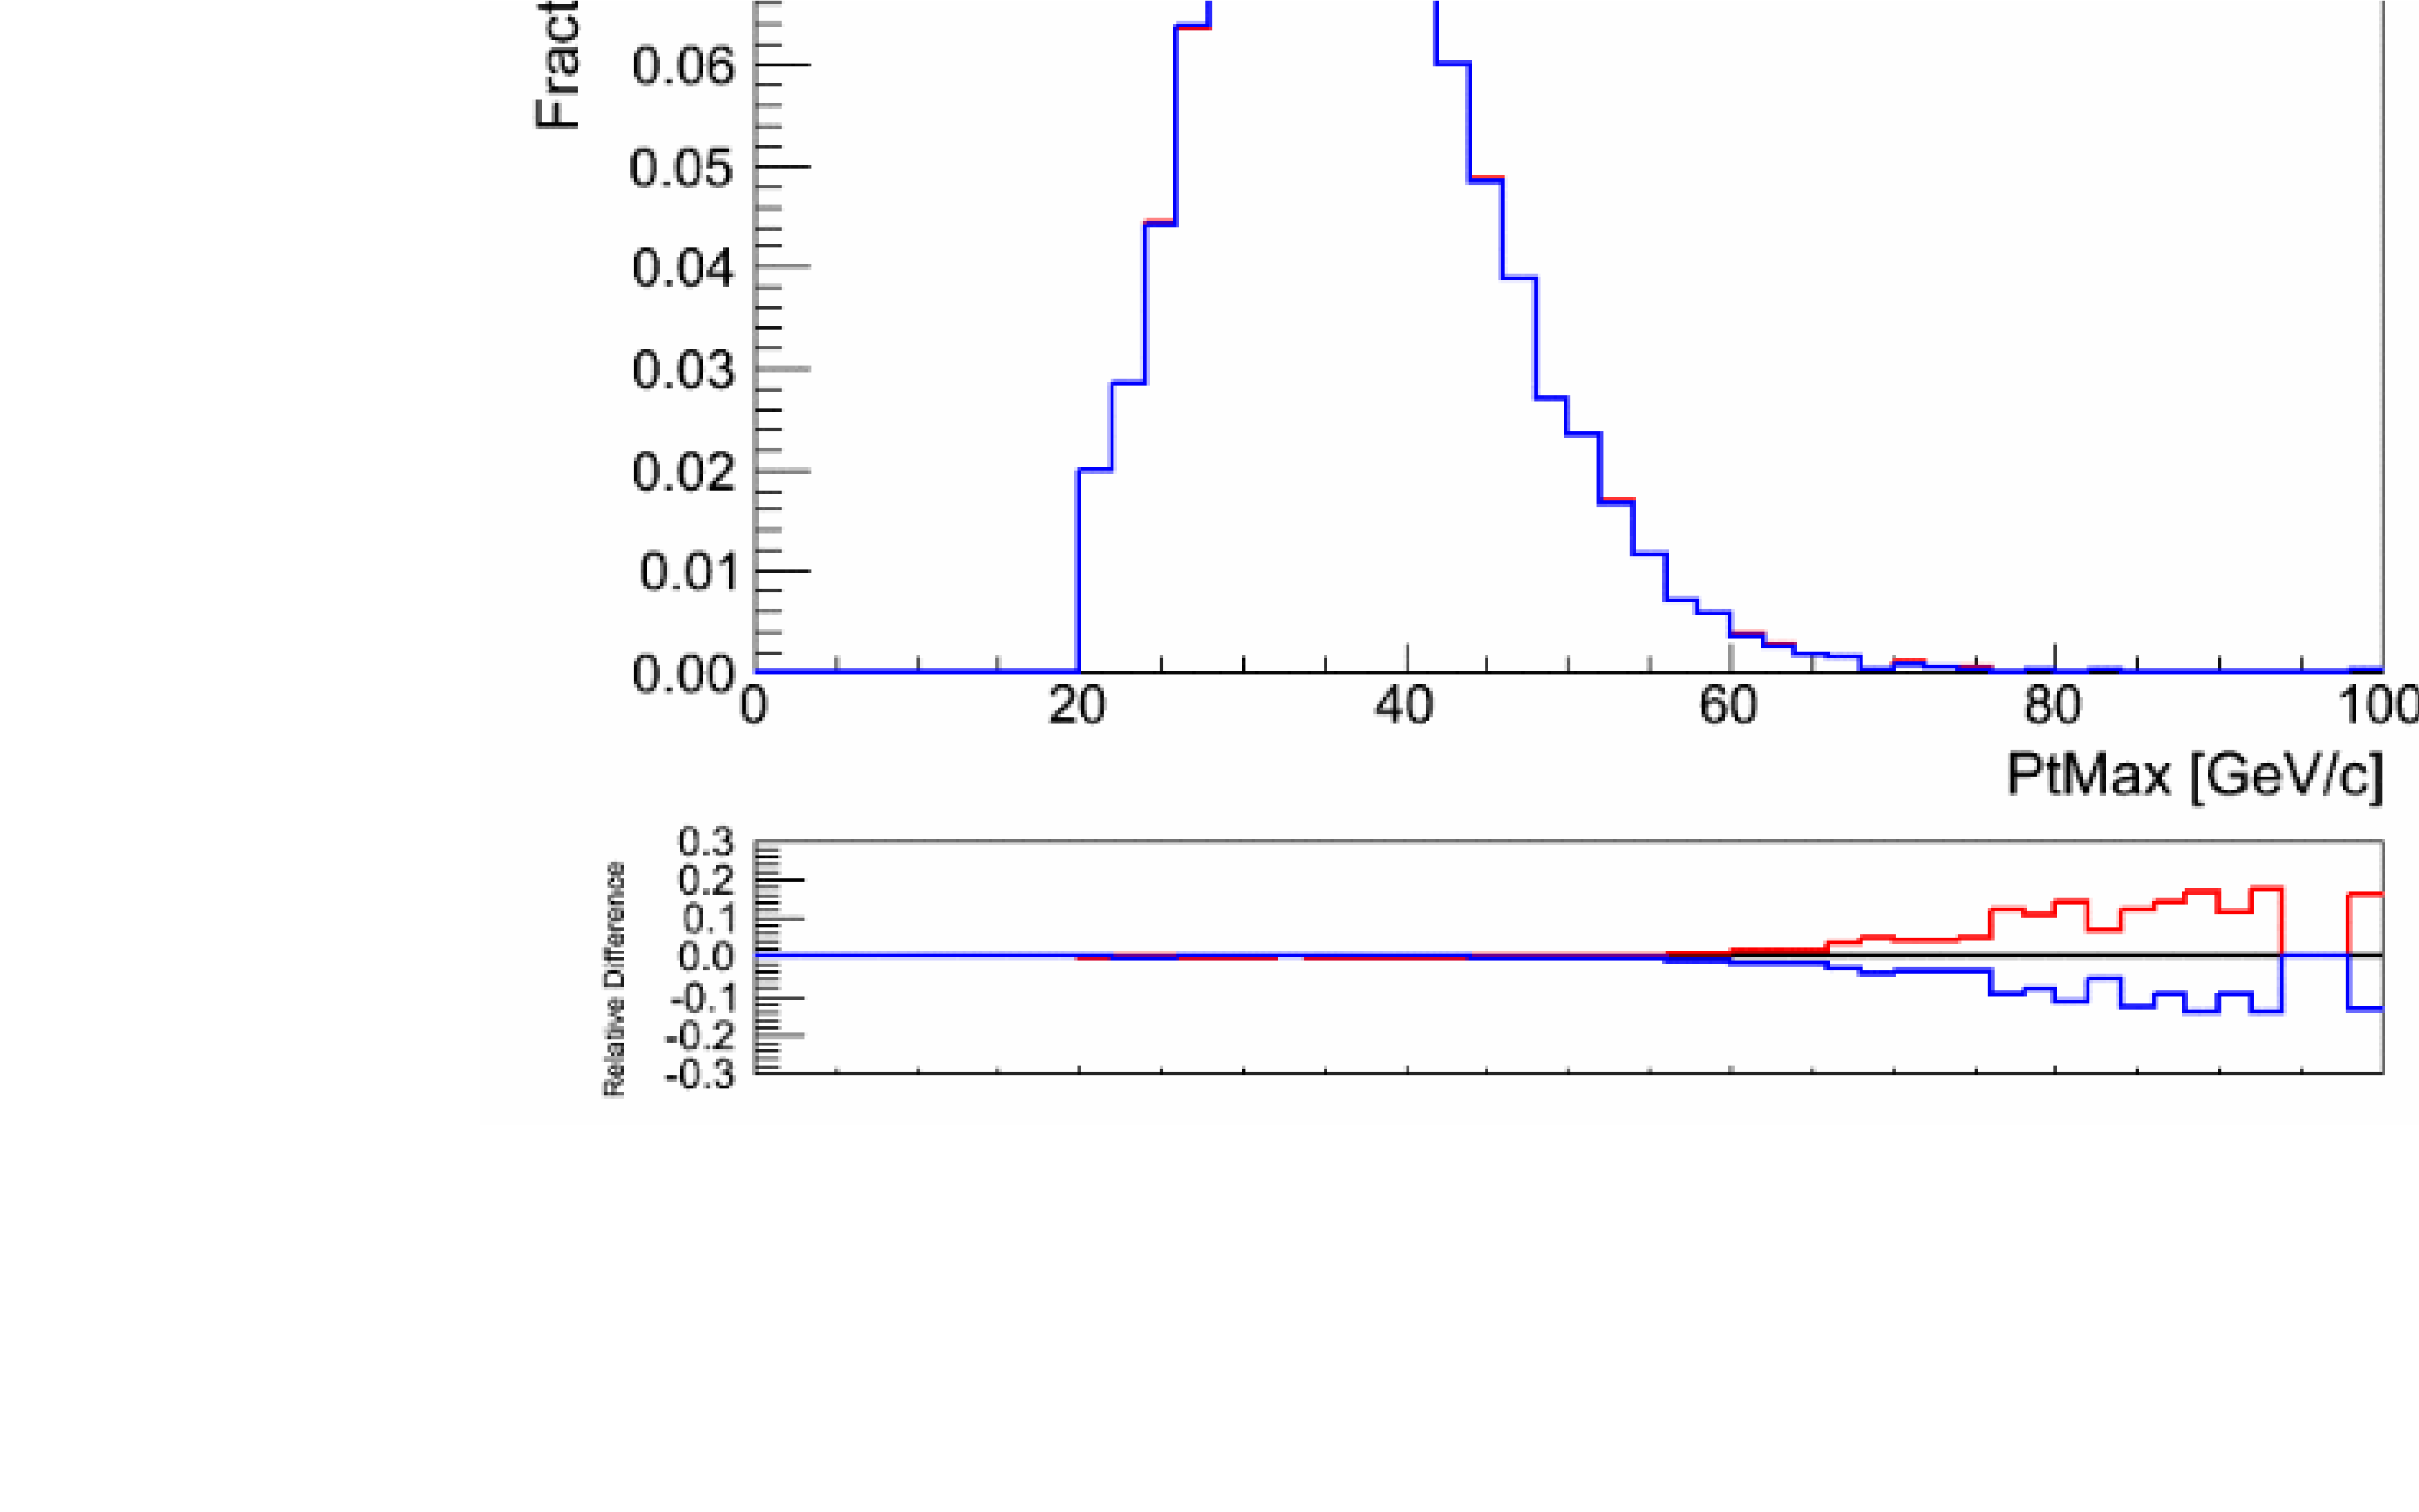
\includegraphics[width=0.49\textwidth]{figures/ShapeSystematics_HWW_PtMax_HQTScaleVariation.pdf}}
\subfigure[PtMax]{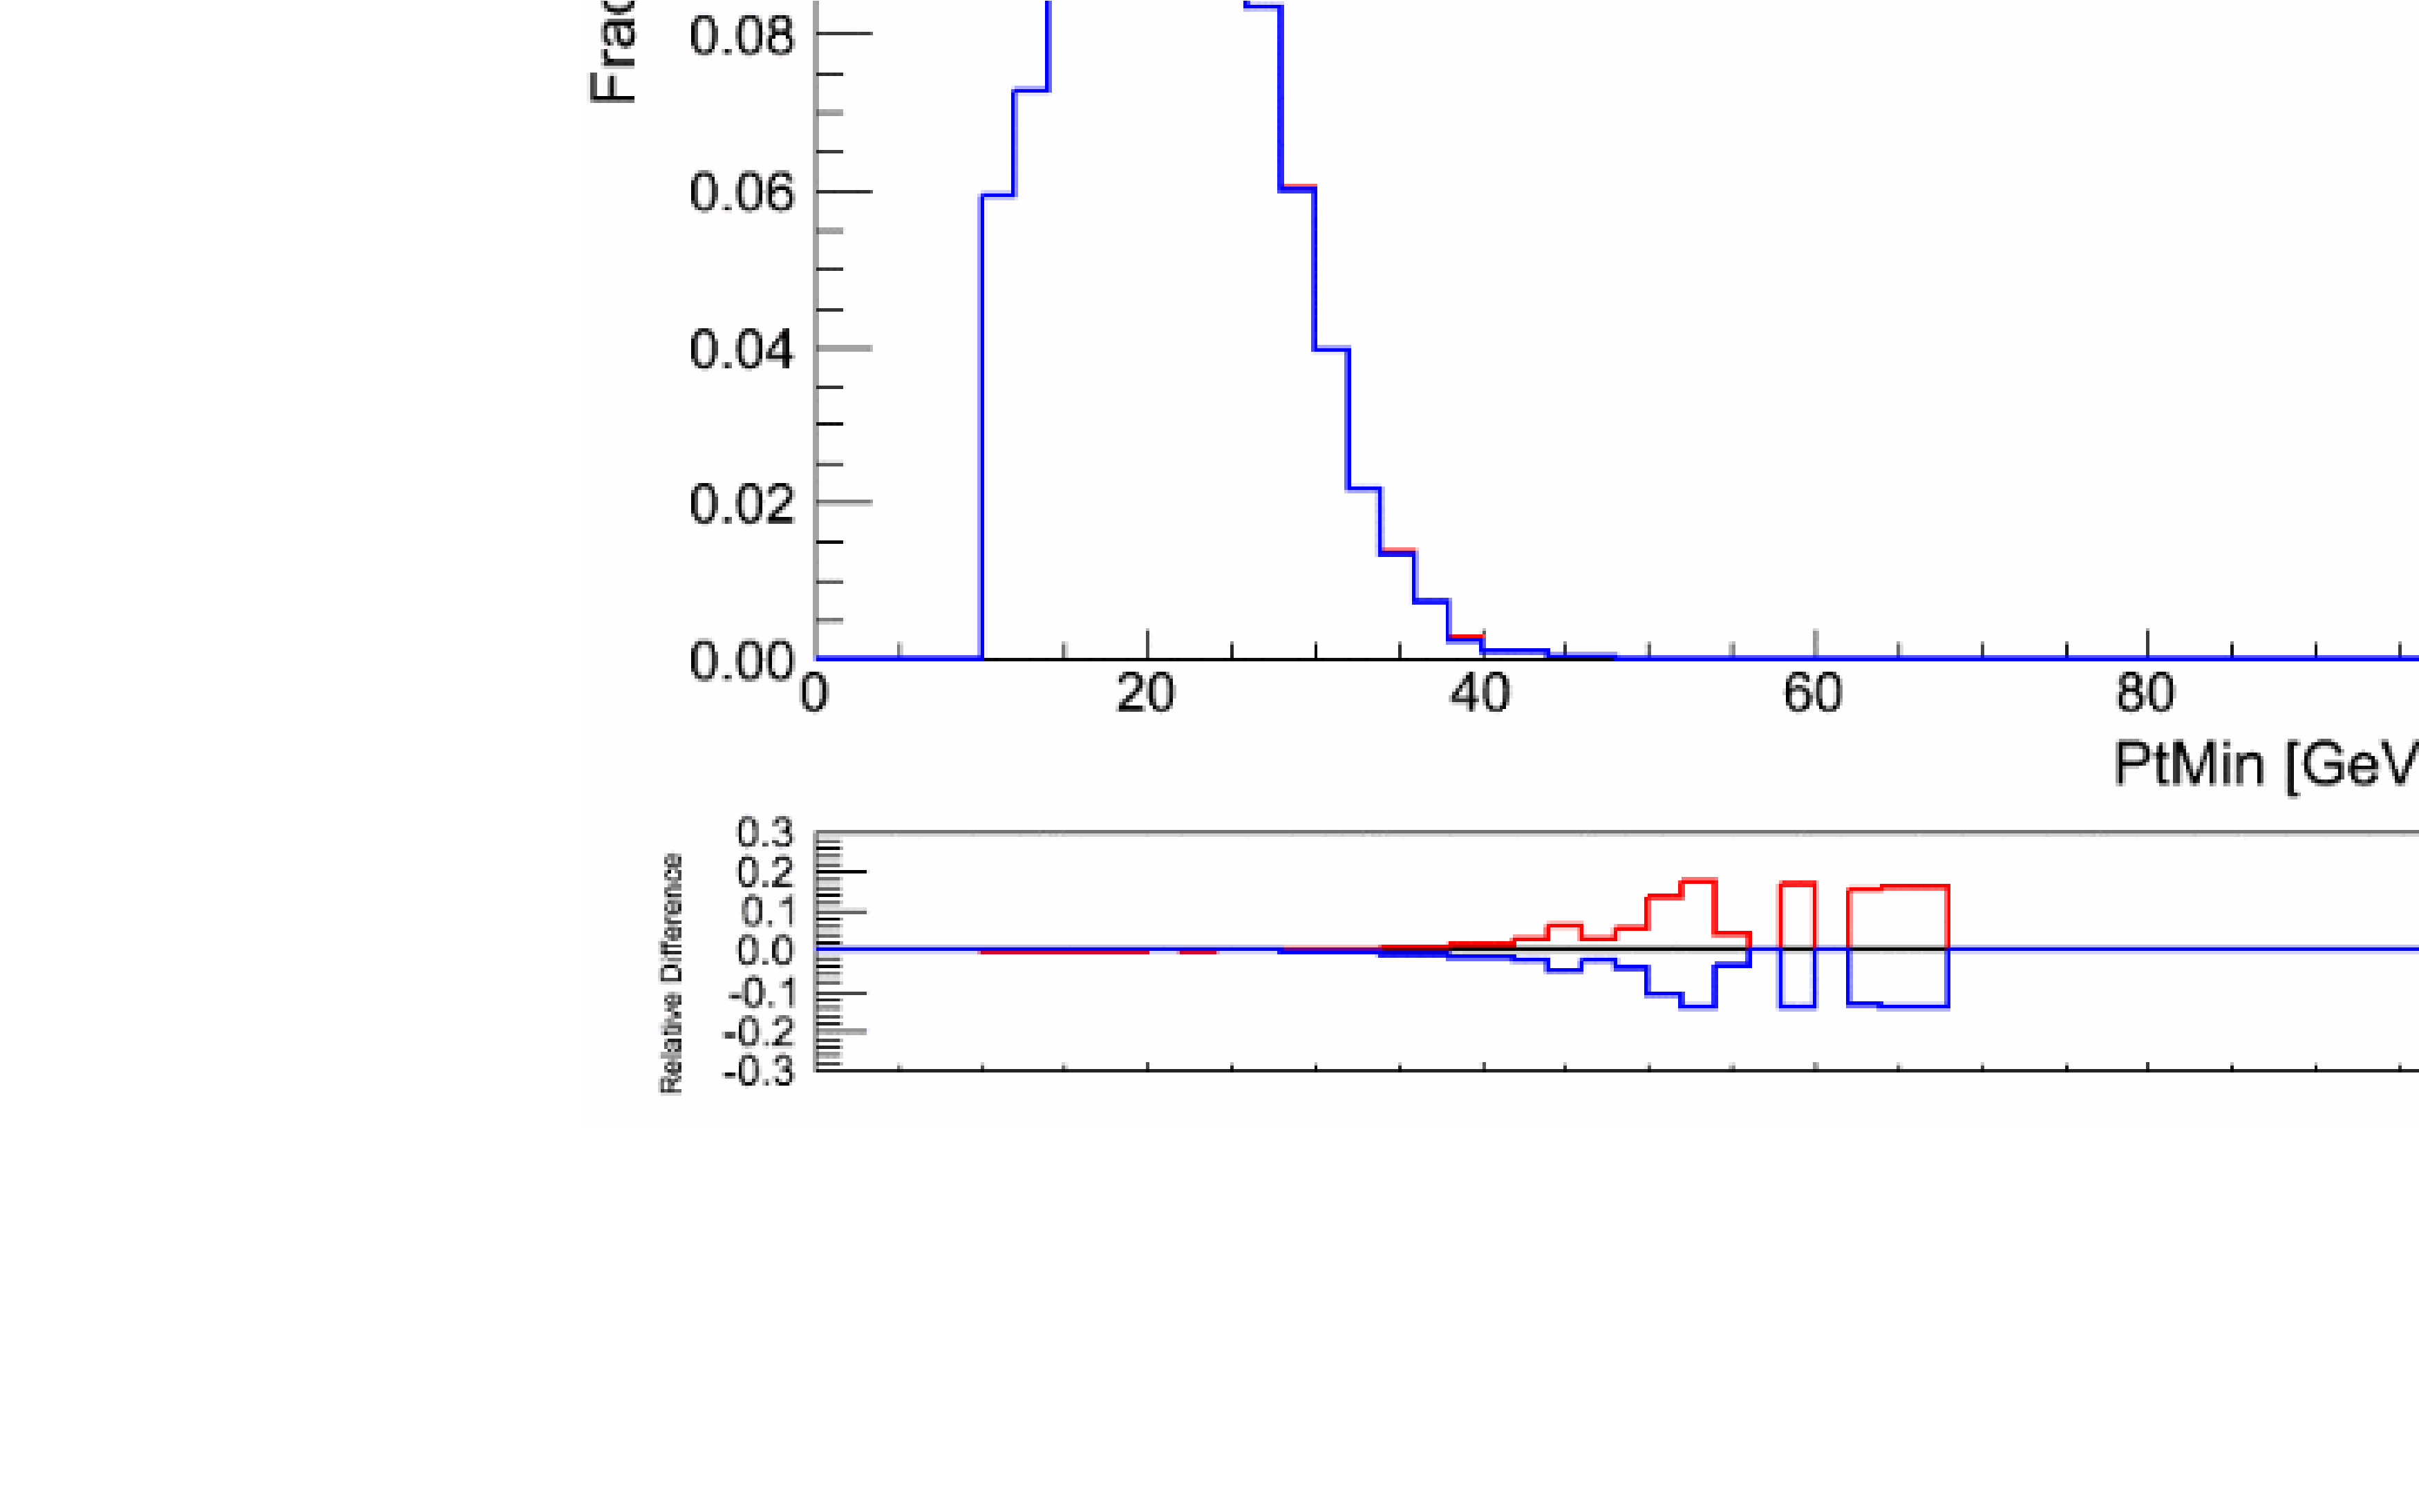
\includegraphics[width=0.49\textwidth]{figures/ShapeSystematics_HWW_PtMin_HQTScaleVariation.pdf}} \\
\subfigure[$M_{\mathrm{T Higgs}}$]{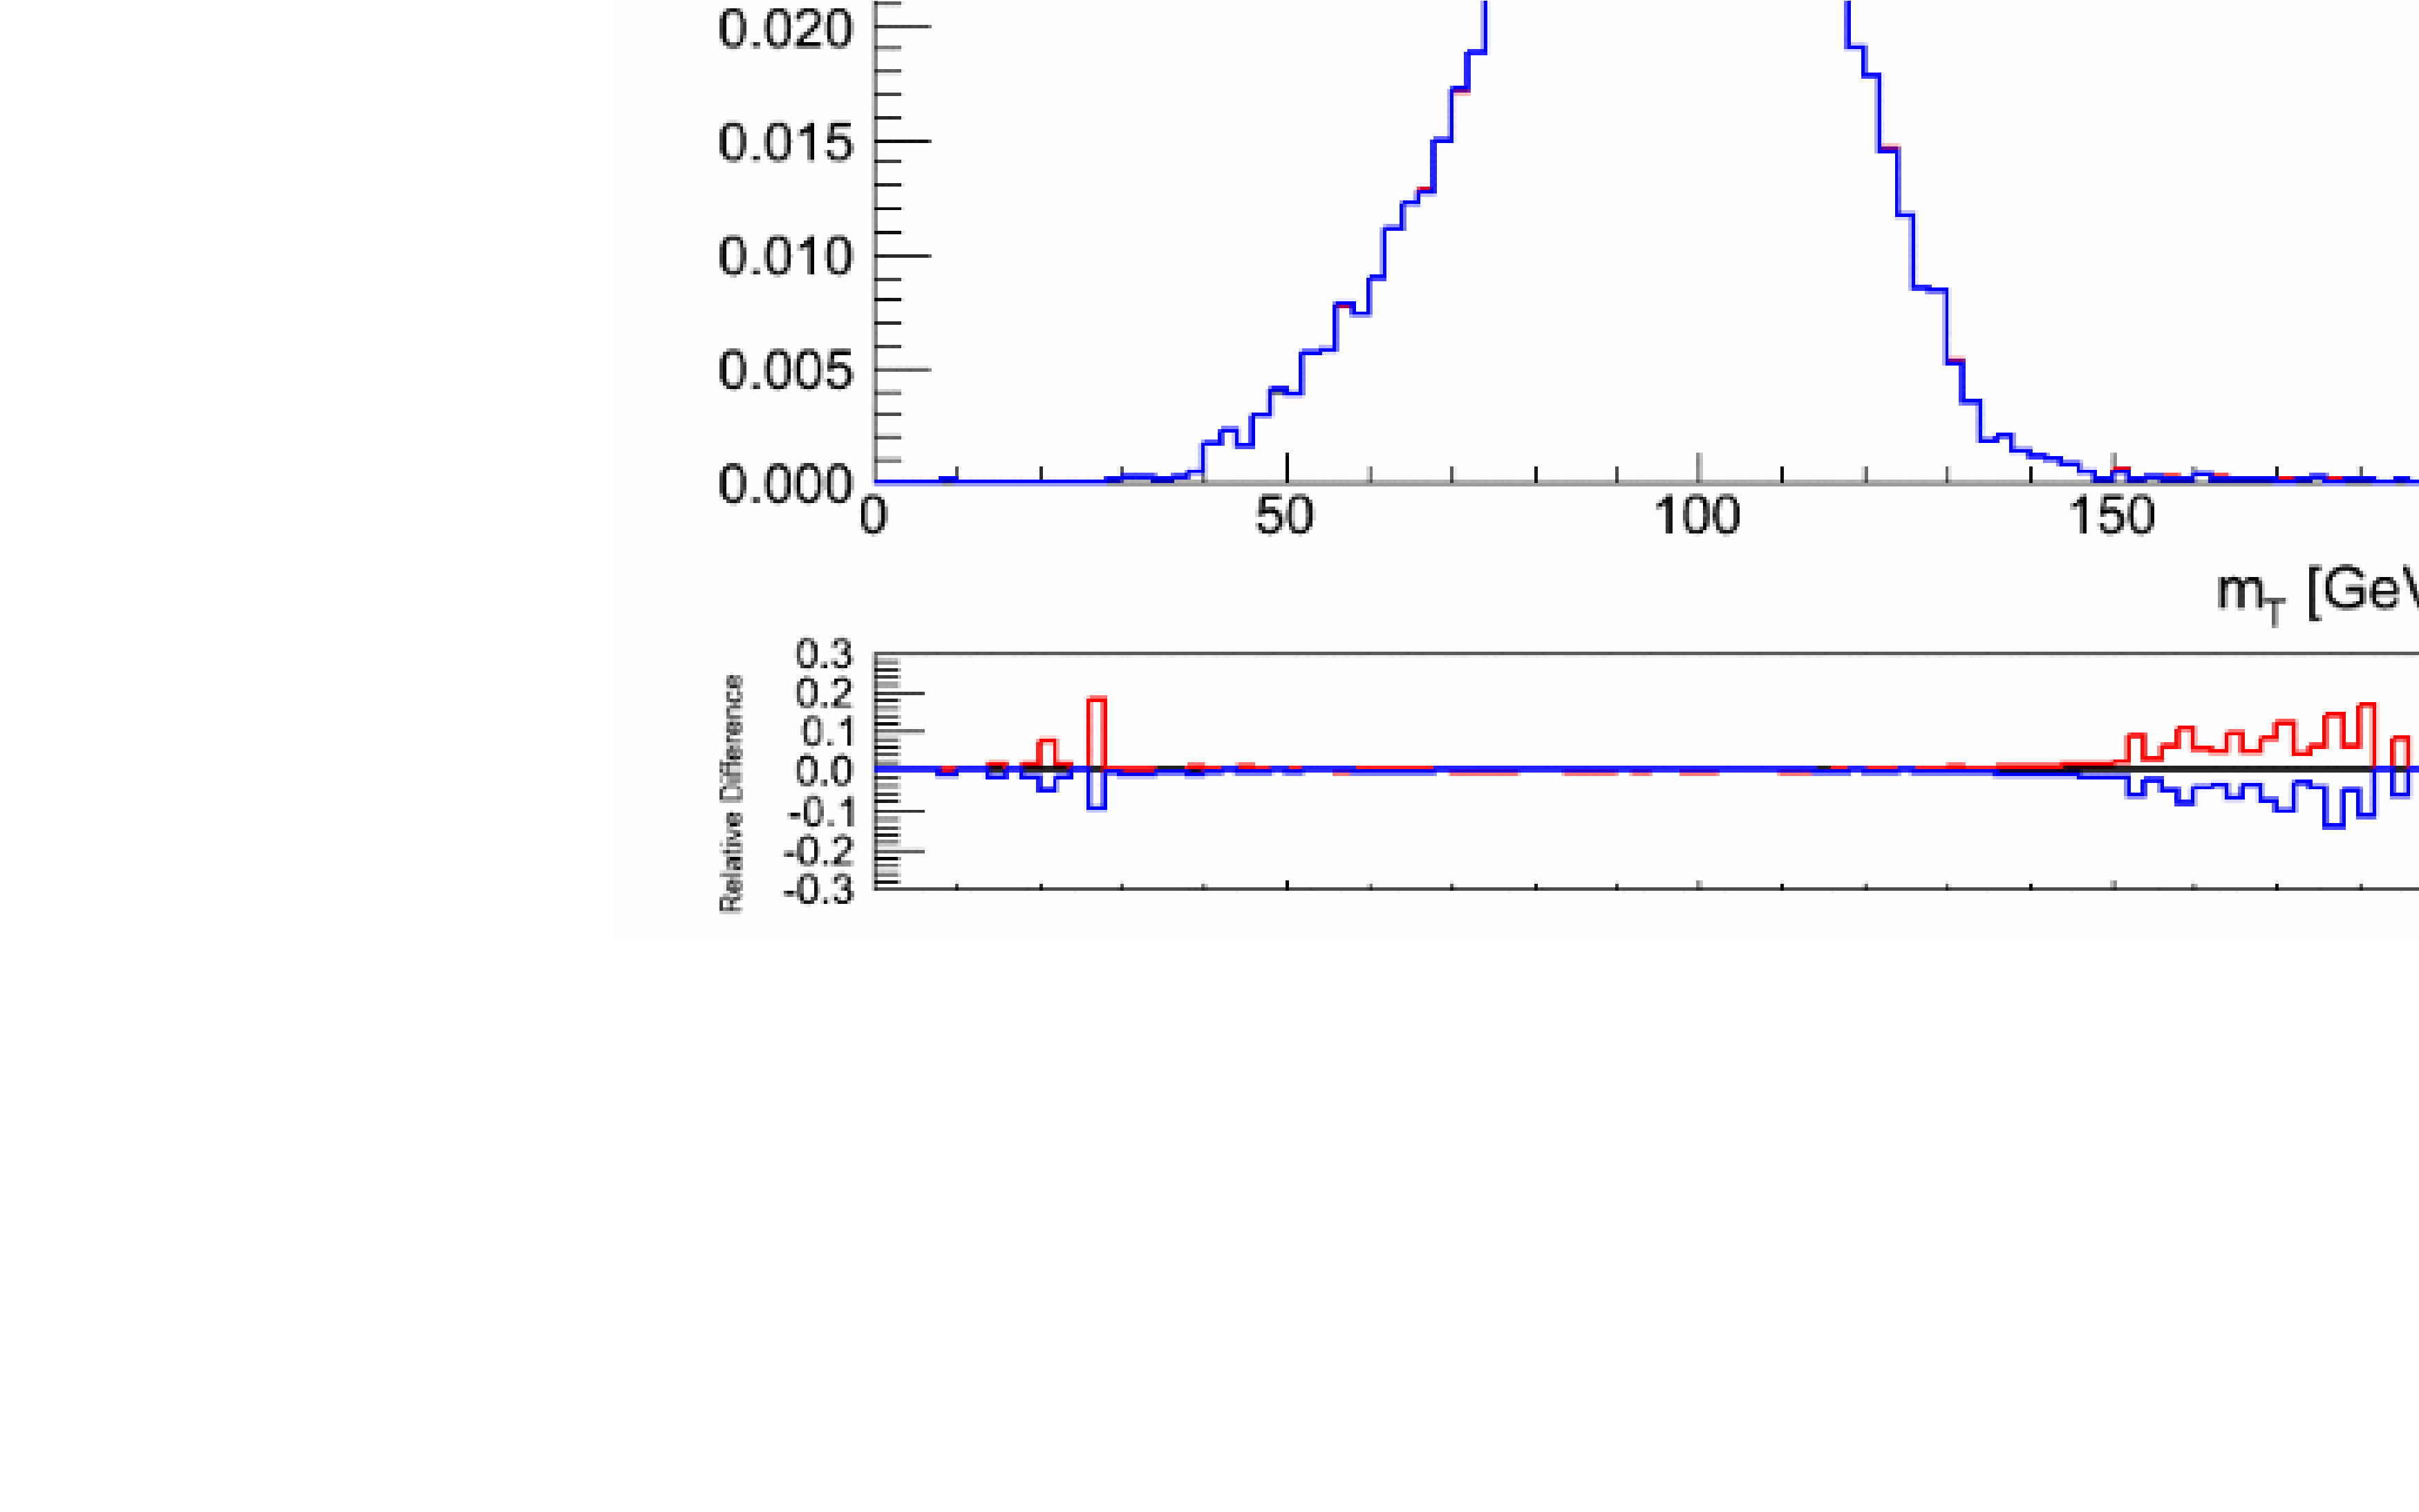
\includegraphics[width=0.49\textwidth]{figures/ShapeSystematics_HWW_MTHiggs_HQTScaleVariation.pdf}}
\subfigure[$\Delta\phi_{\mathrm{ll}}$]{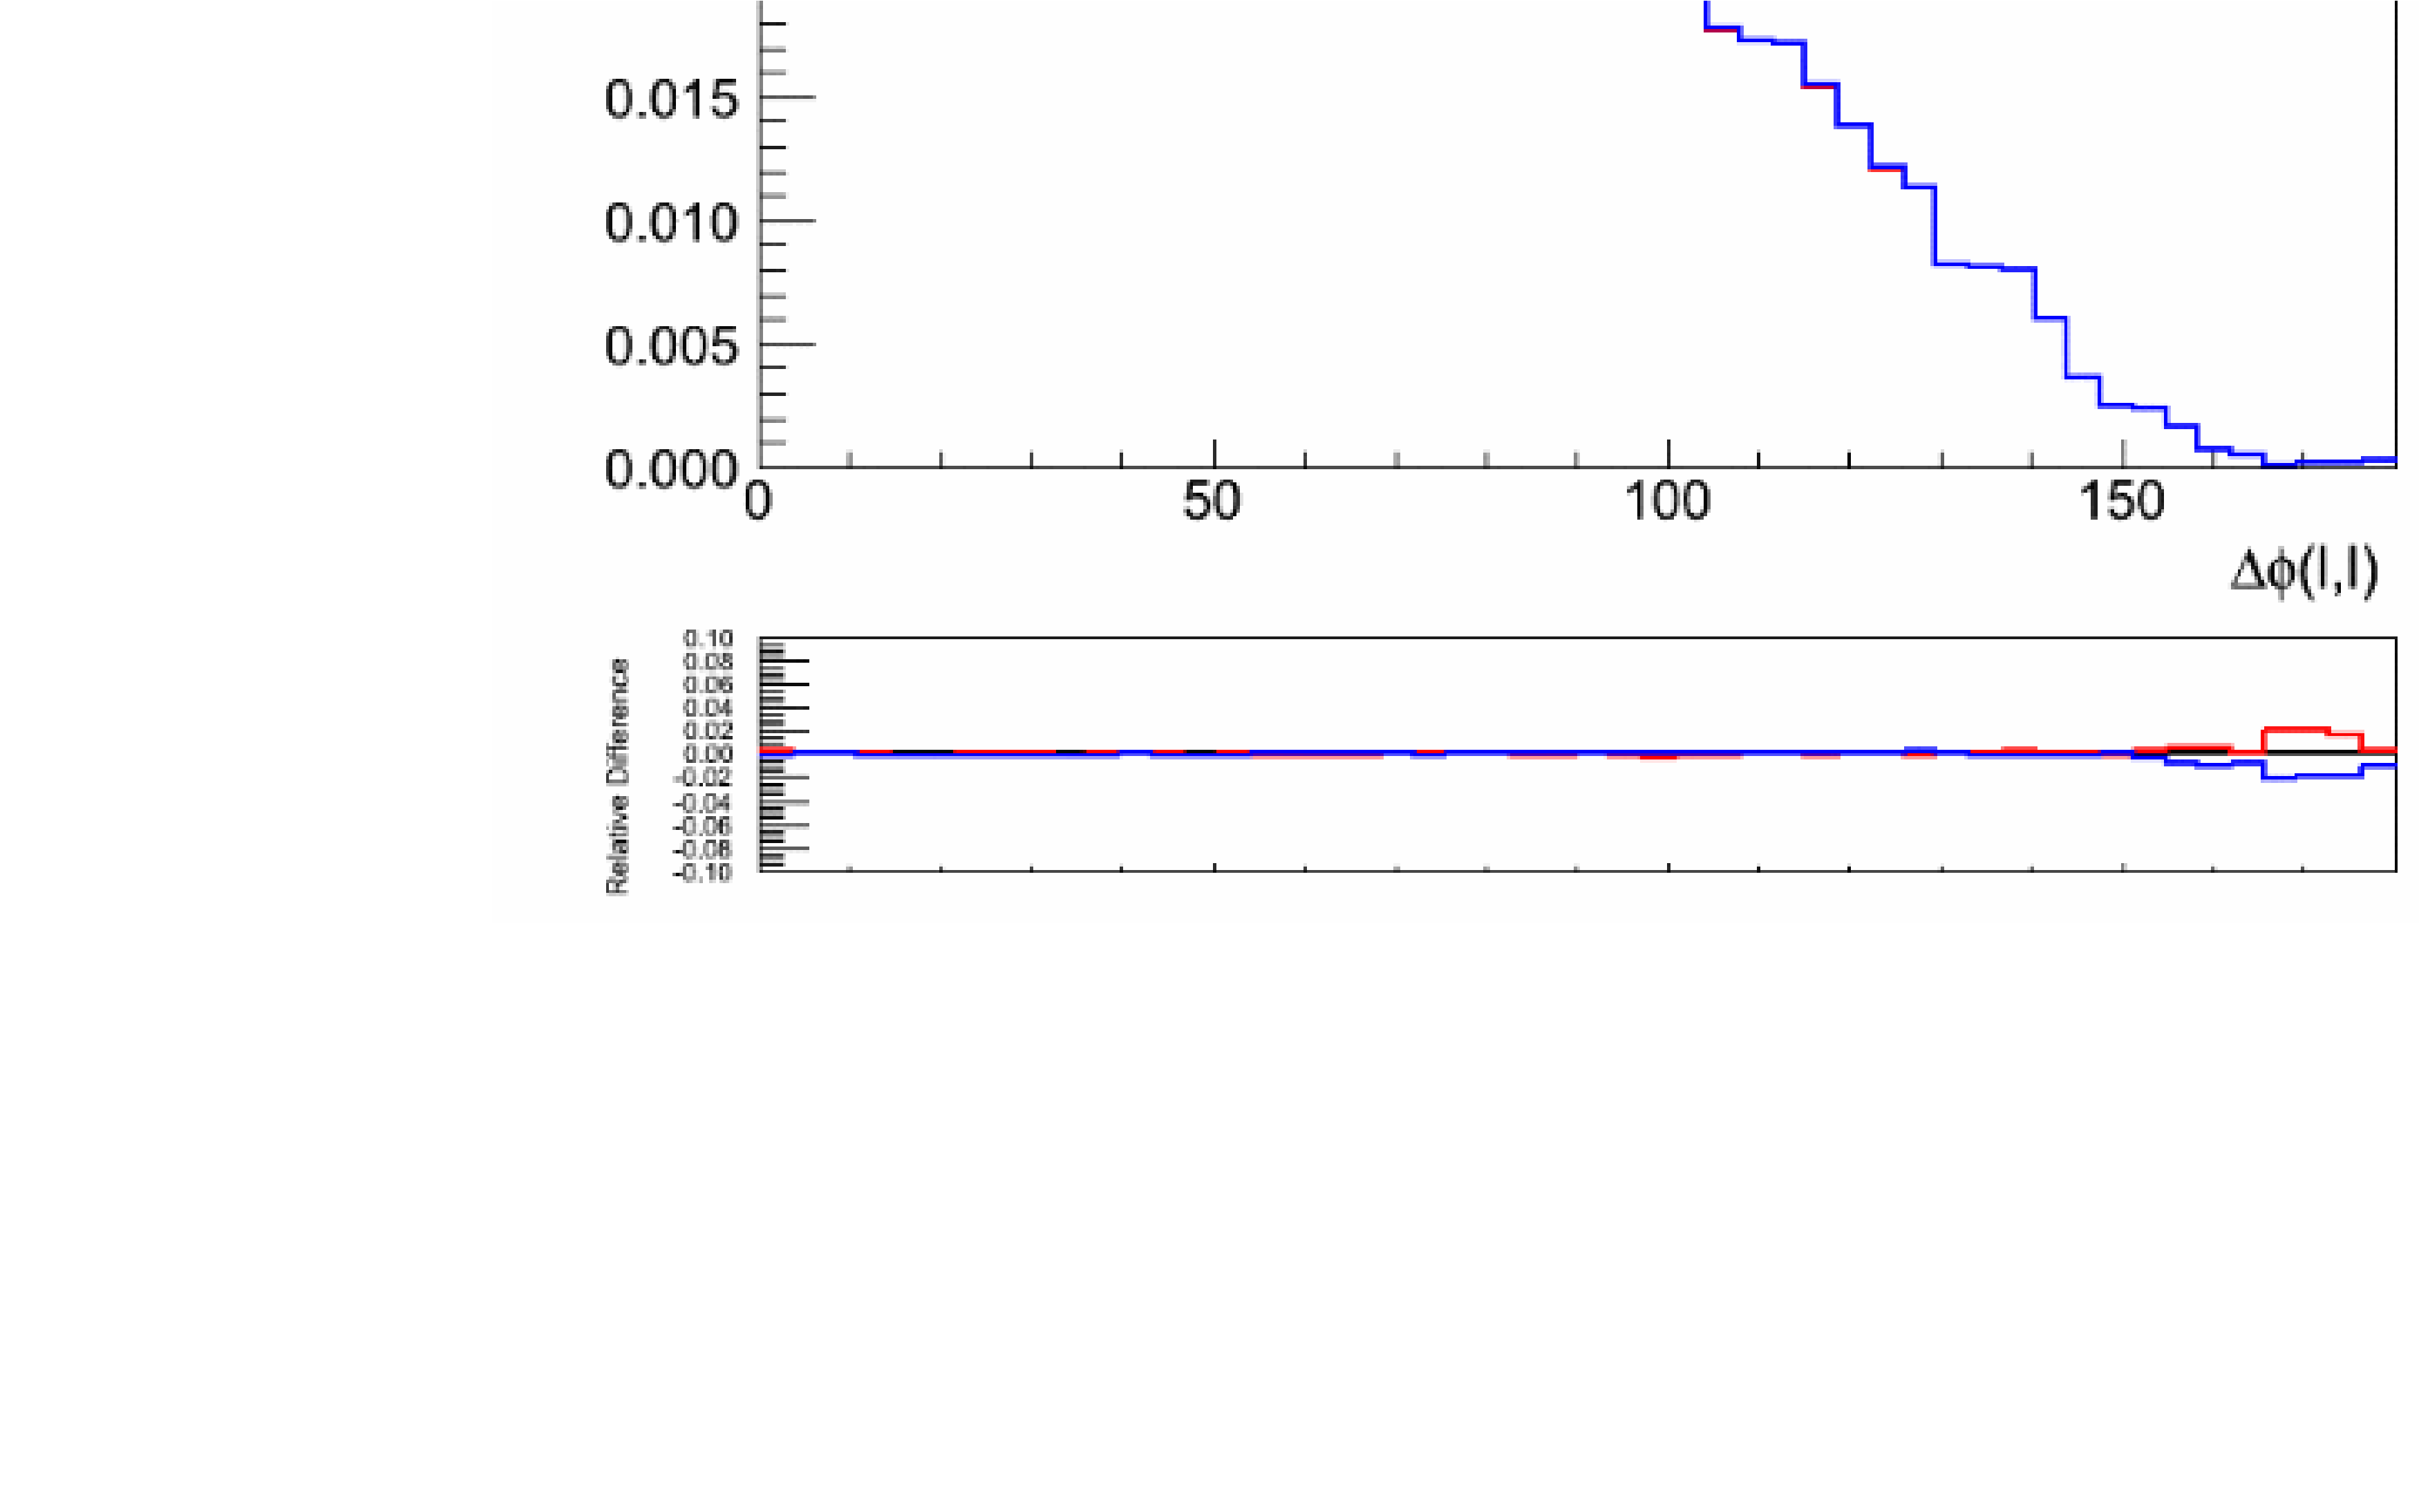
\includegraphics[width=0.49\textwidth]{figures/ShapeSystematics_HWW_DeltaPhi_HQTScaleVariation.pdf}}
\caption{Comparison of the four most discriminant MVA input variables between the prediction of the MC
reweighted to the scale varied and default $p_{T}$ spectra. 
}
\label{fig:signalshape_PtSpectrumScaleVariation_InputObservables}
\end{center}
\end{figure}
%%%%%%%%%%%%%%%%%%%%%%%%%%%%%%%%%%%



%%%%%%%%%%%%%%%%%%%%%%%%%%%%%%%%%%%
\begin{figure}[!htbp]
\begin{center}
\subfigure[$M_{H}=130$GeV MVA]{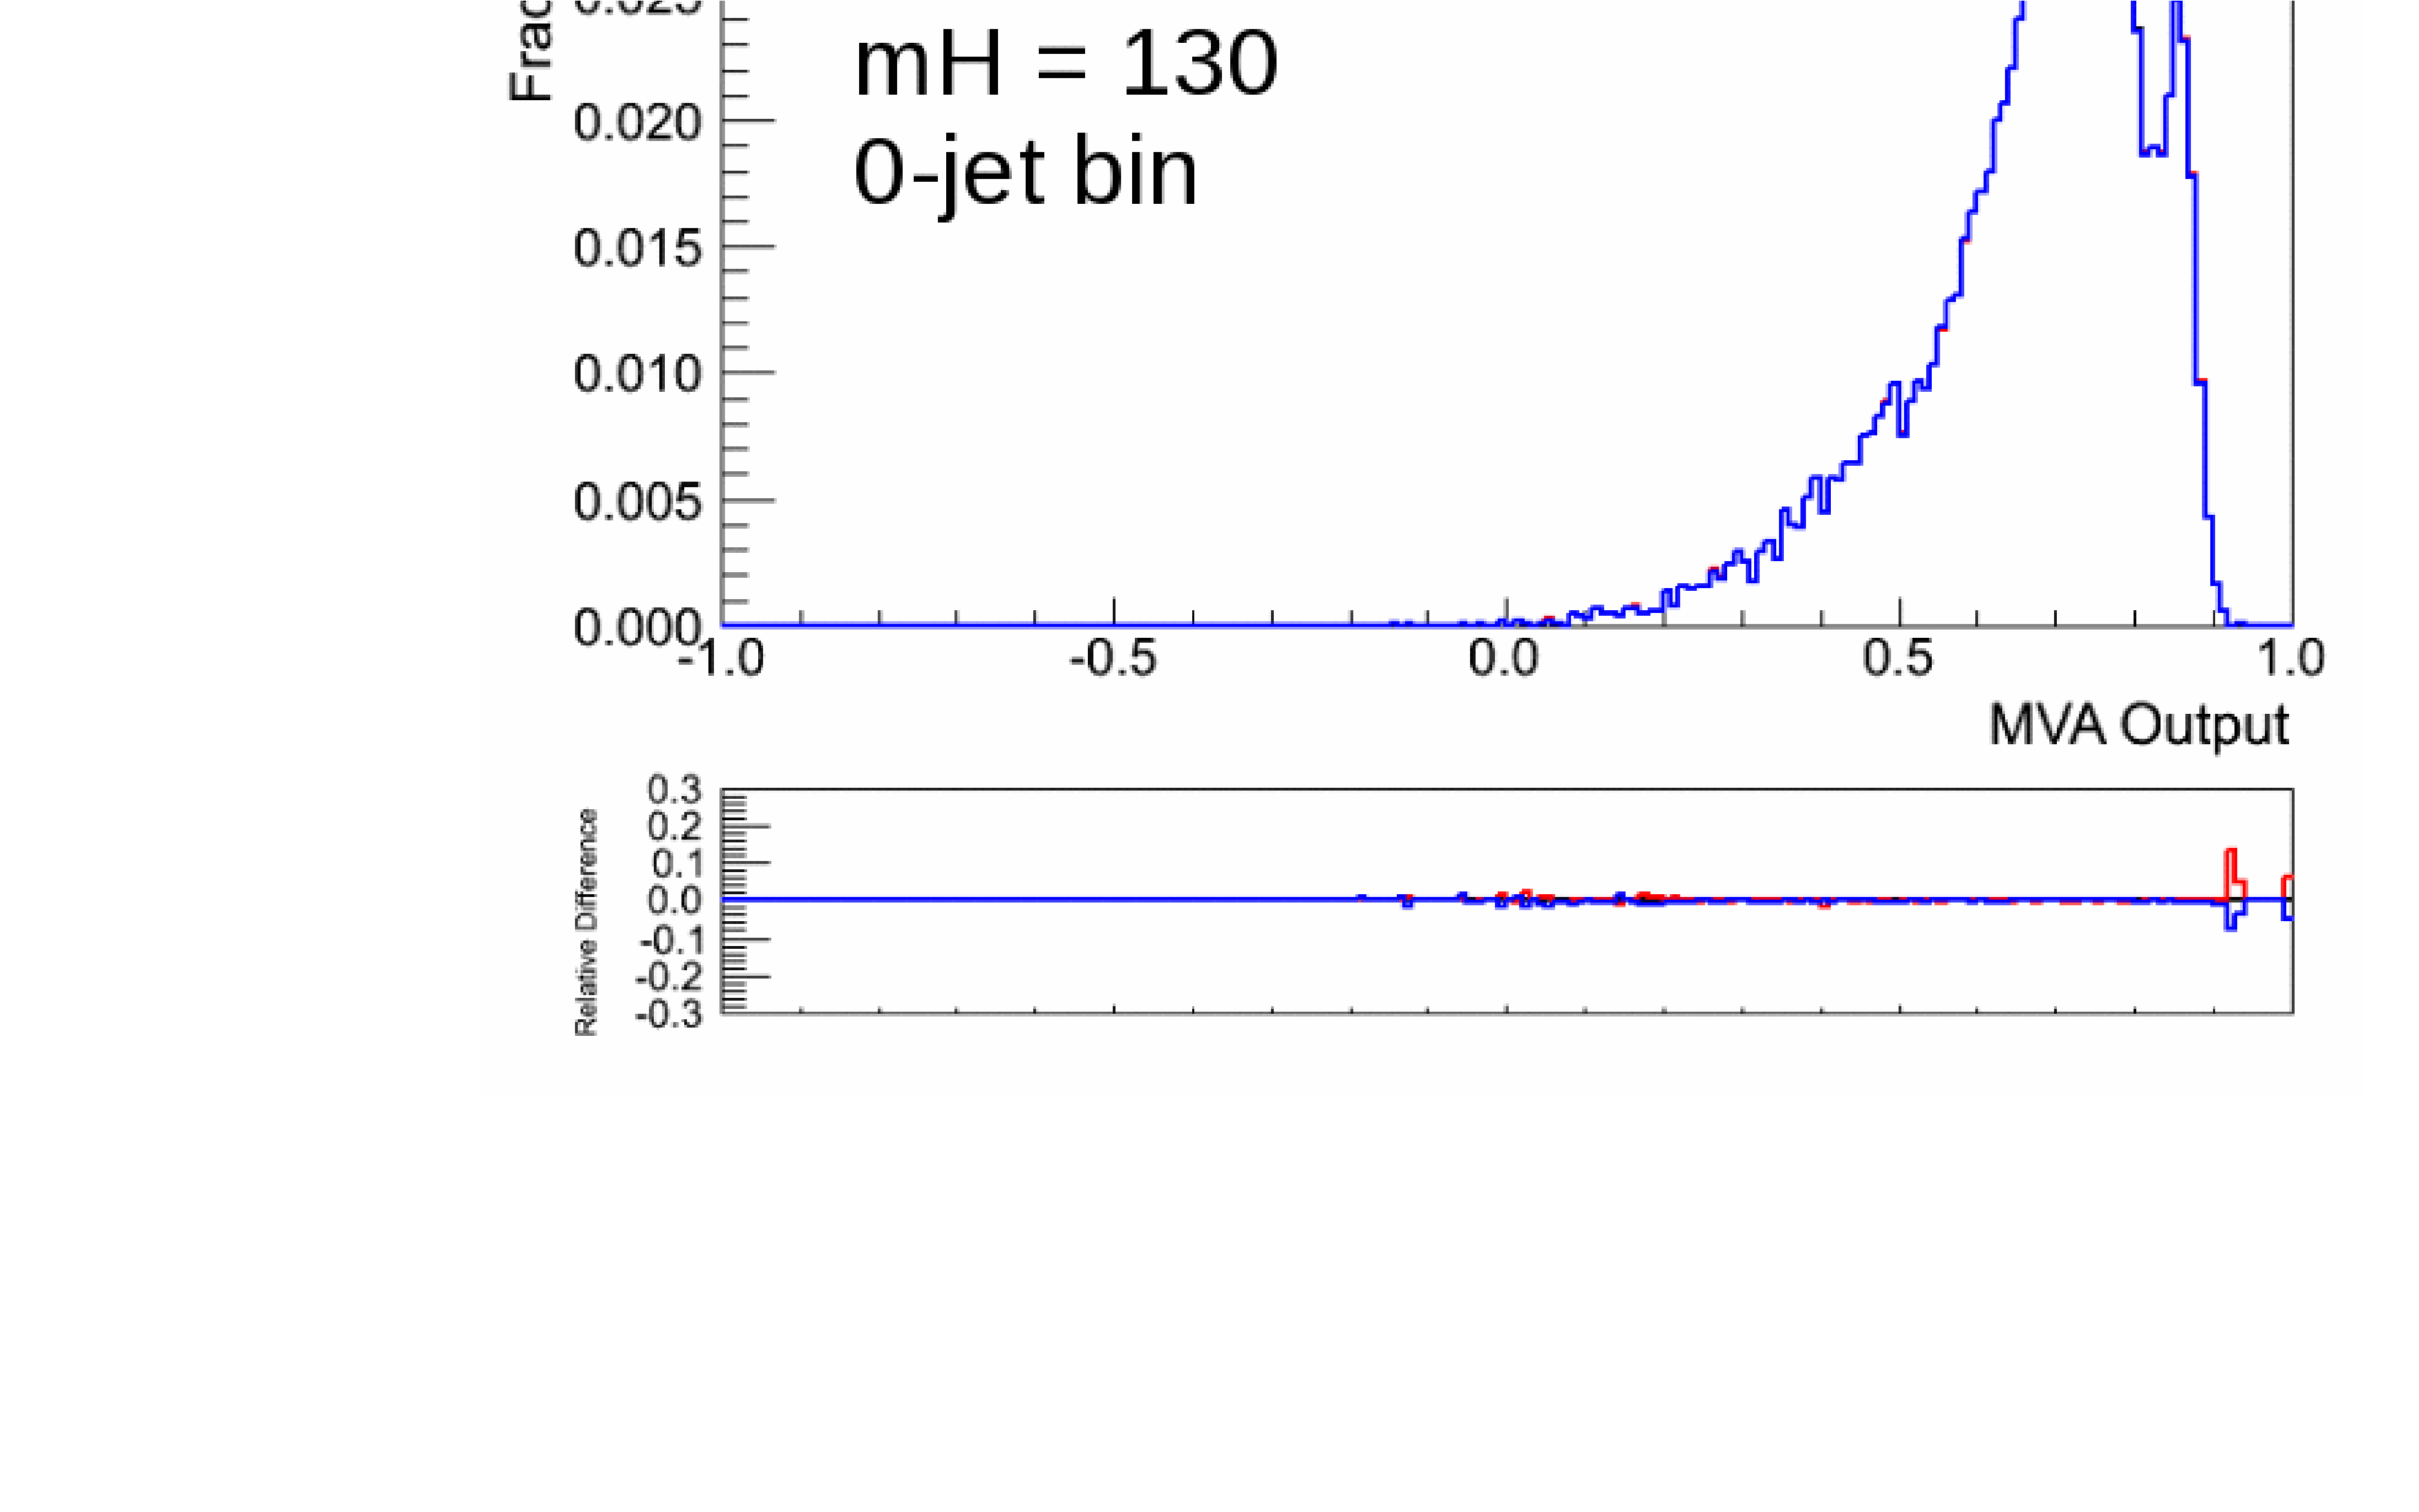
\includegraphics[width=0.49\textwidth]{figures/ShapeSystematics_HWW_MVA130_HQTScaleVariation.pdf}}
\subfigure[$M_{H}=160$GeV MVA]{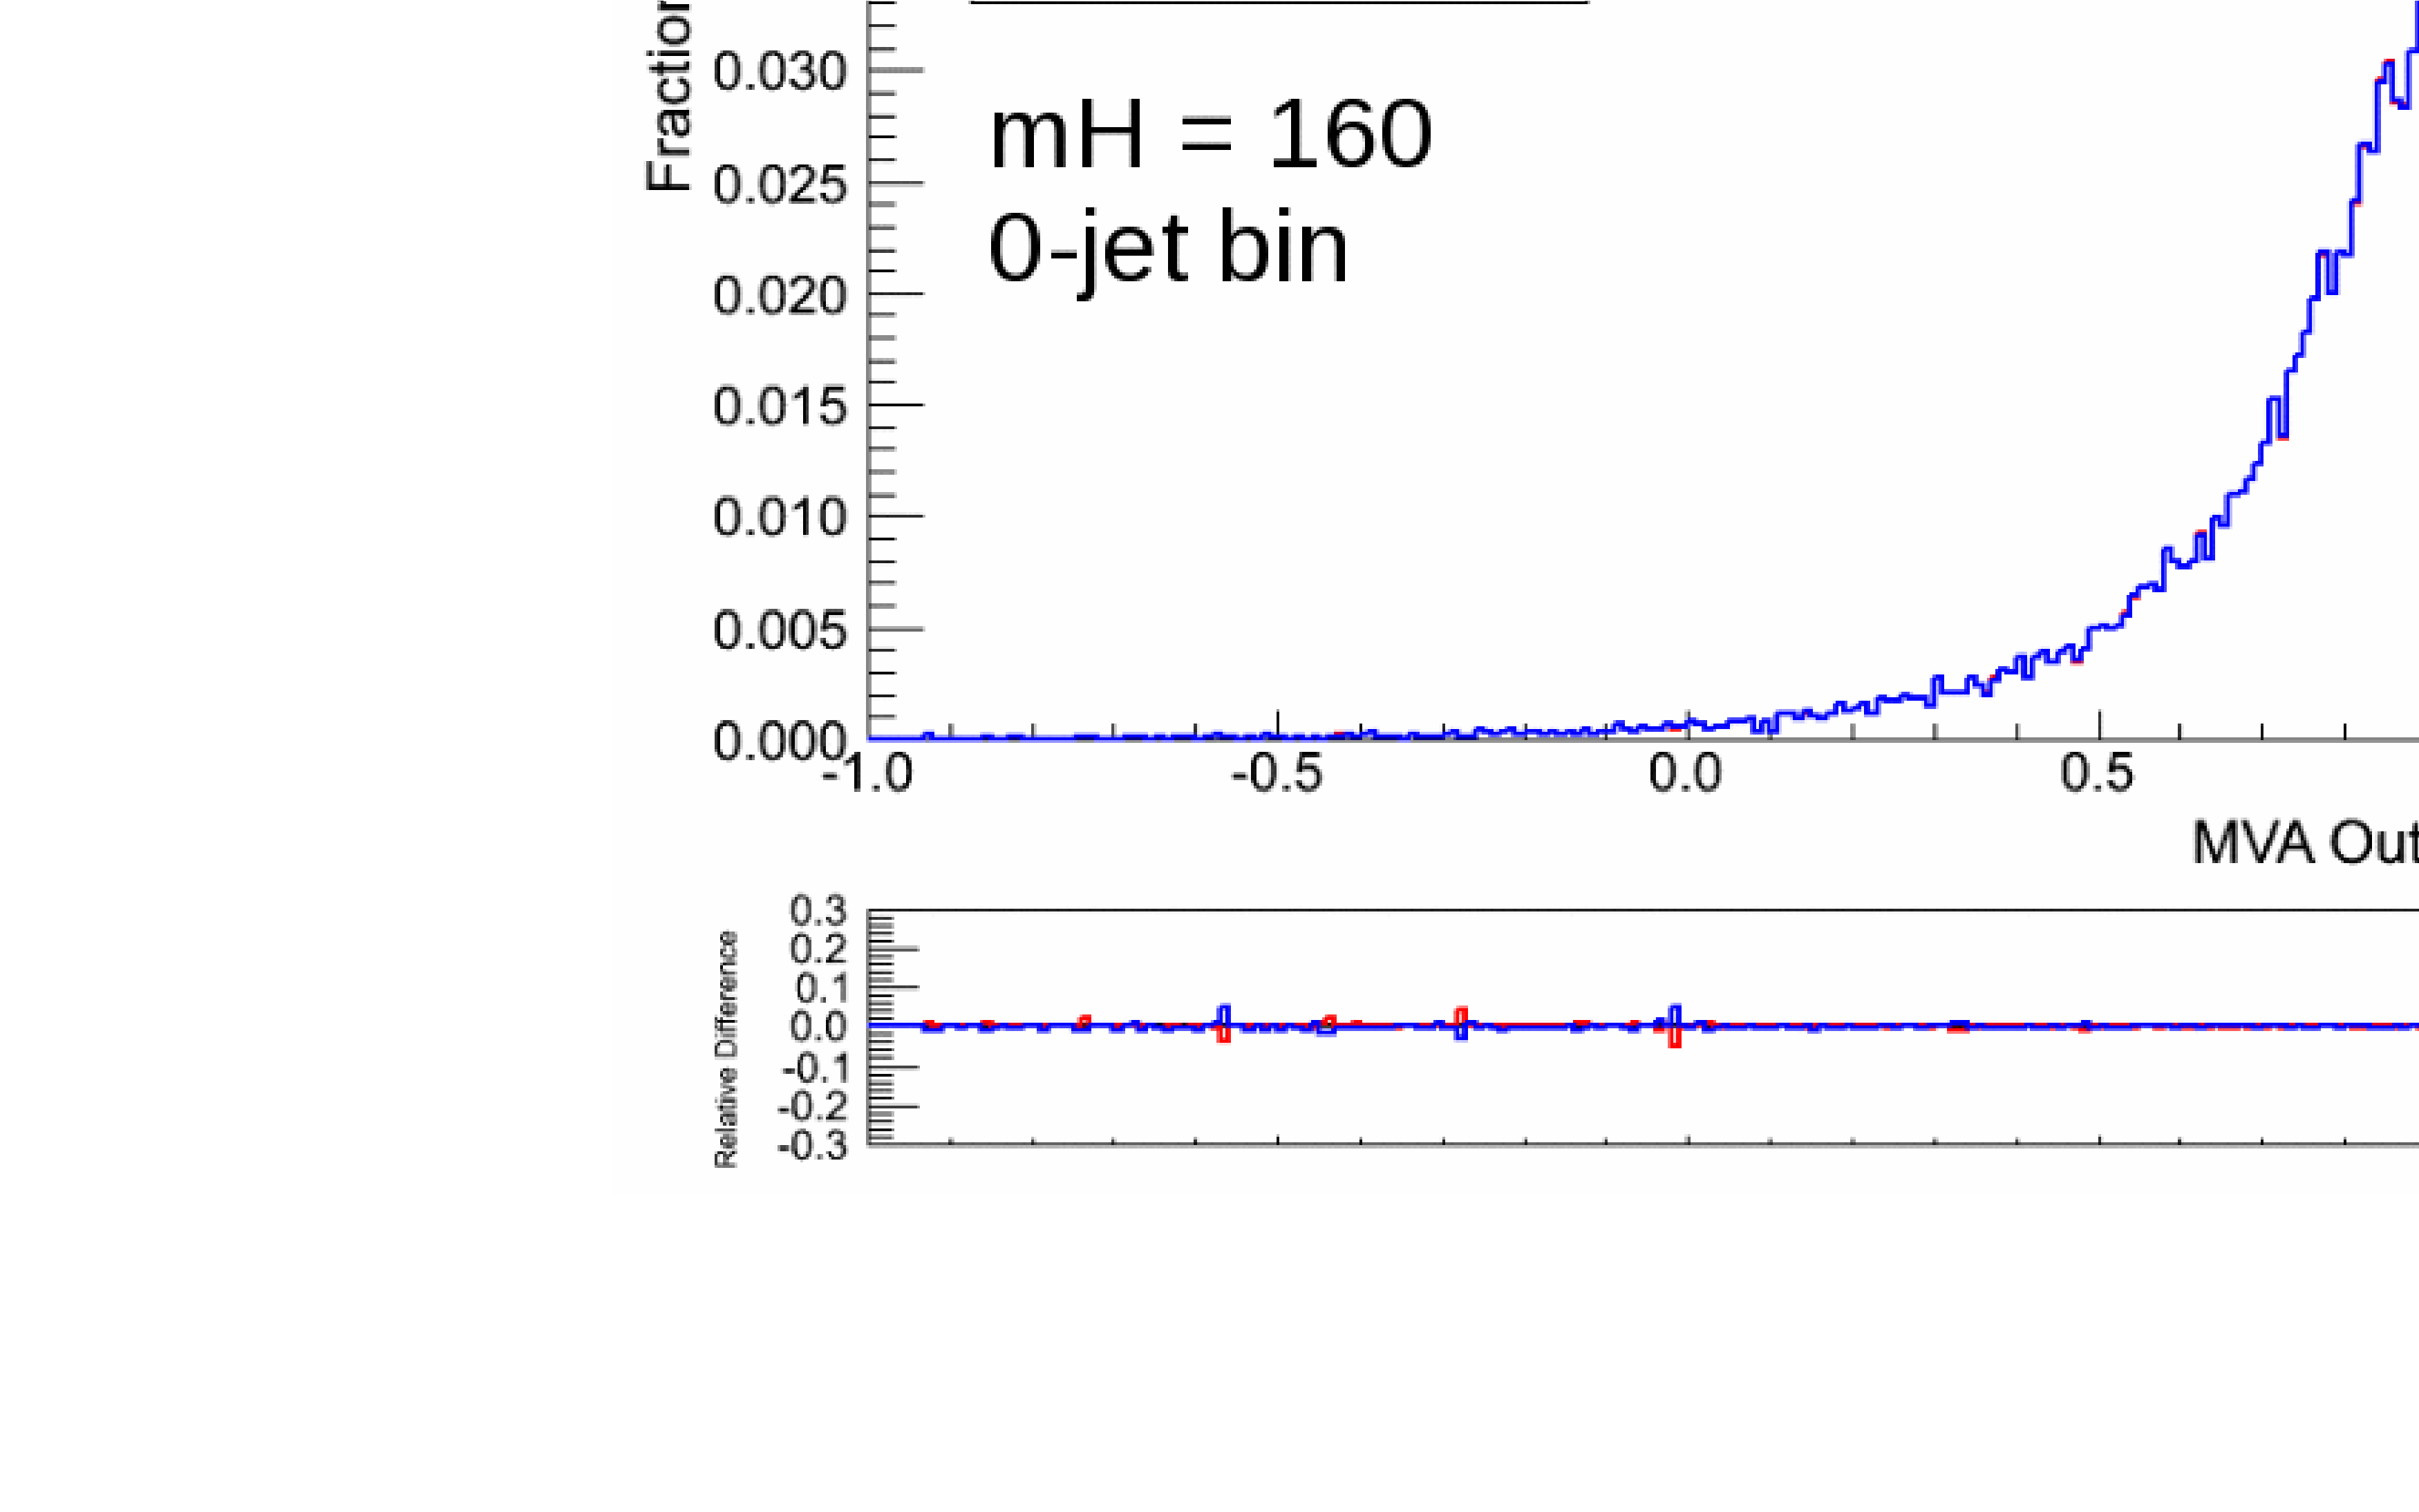
\includegraphics[width=0.49\textwidth]{figures/ShapeSystematics_HWW_MVA160_HQTScaleVariation.pdf}}
\subfigure[$M_{H}=400$GeV MVA]{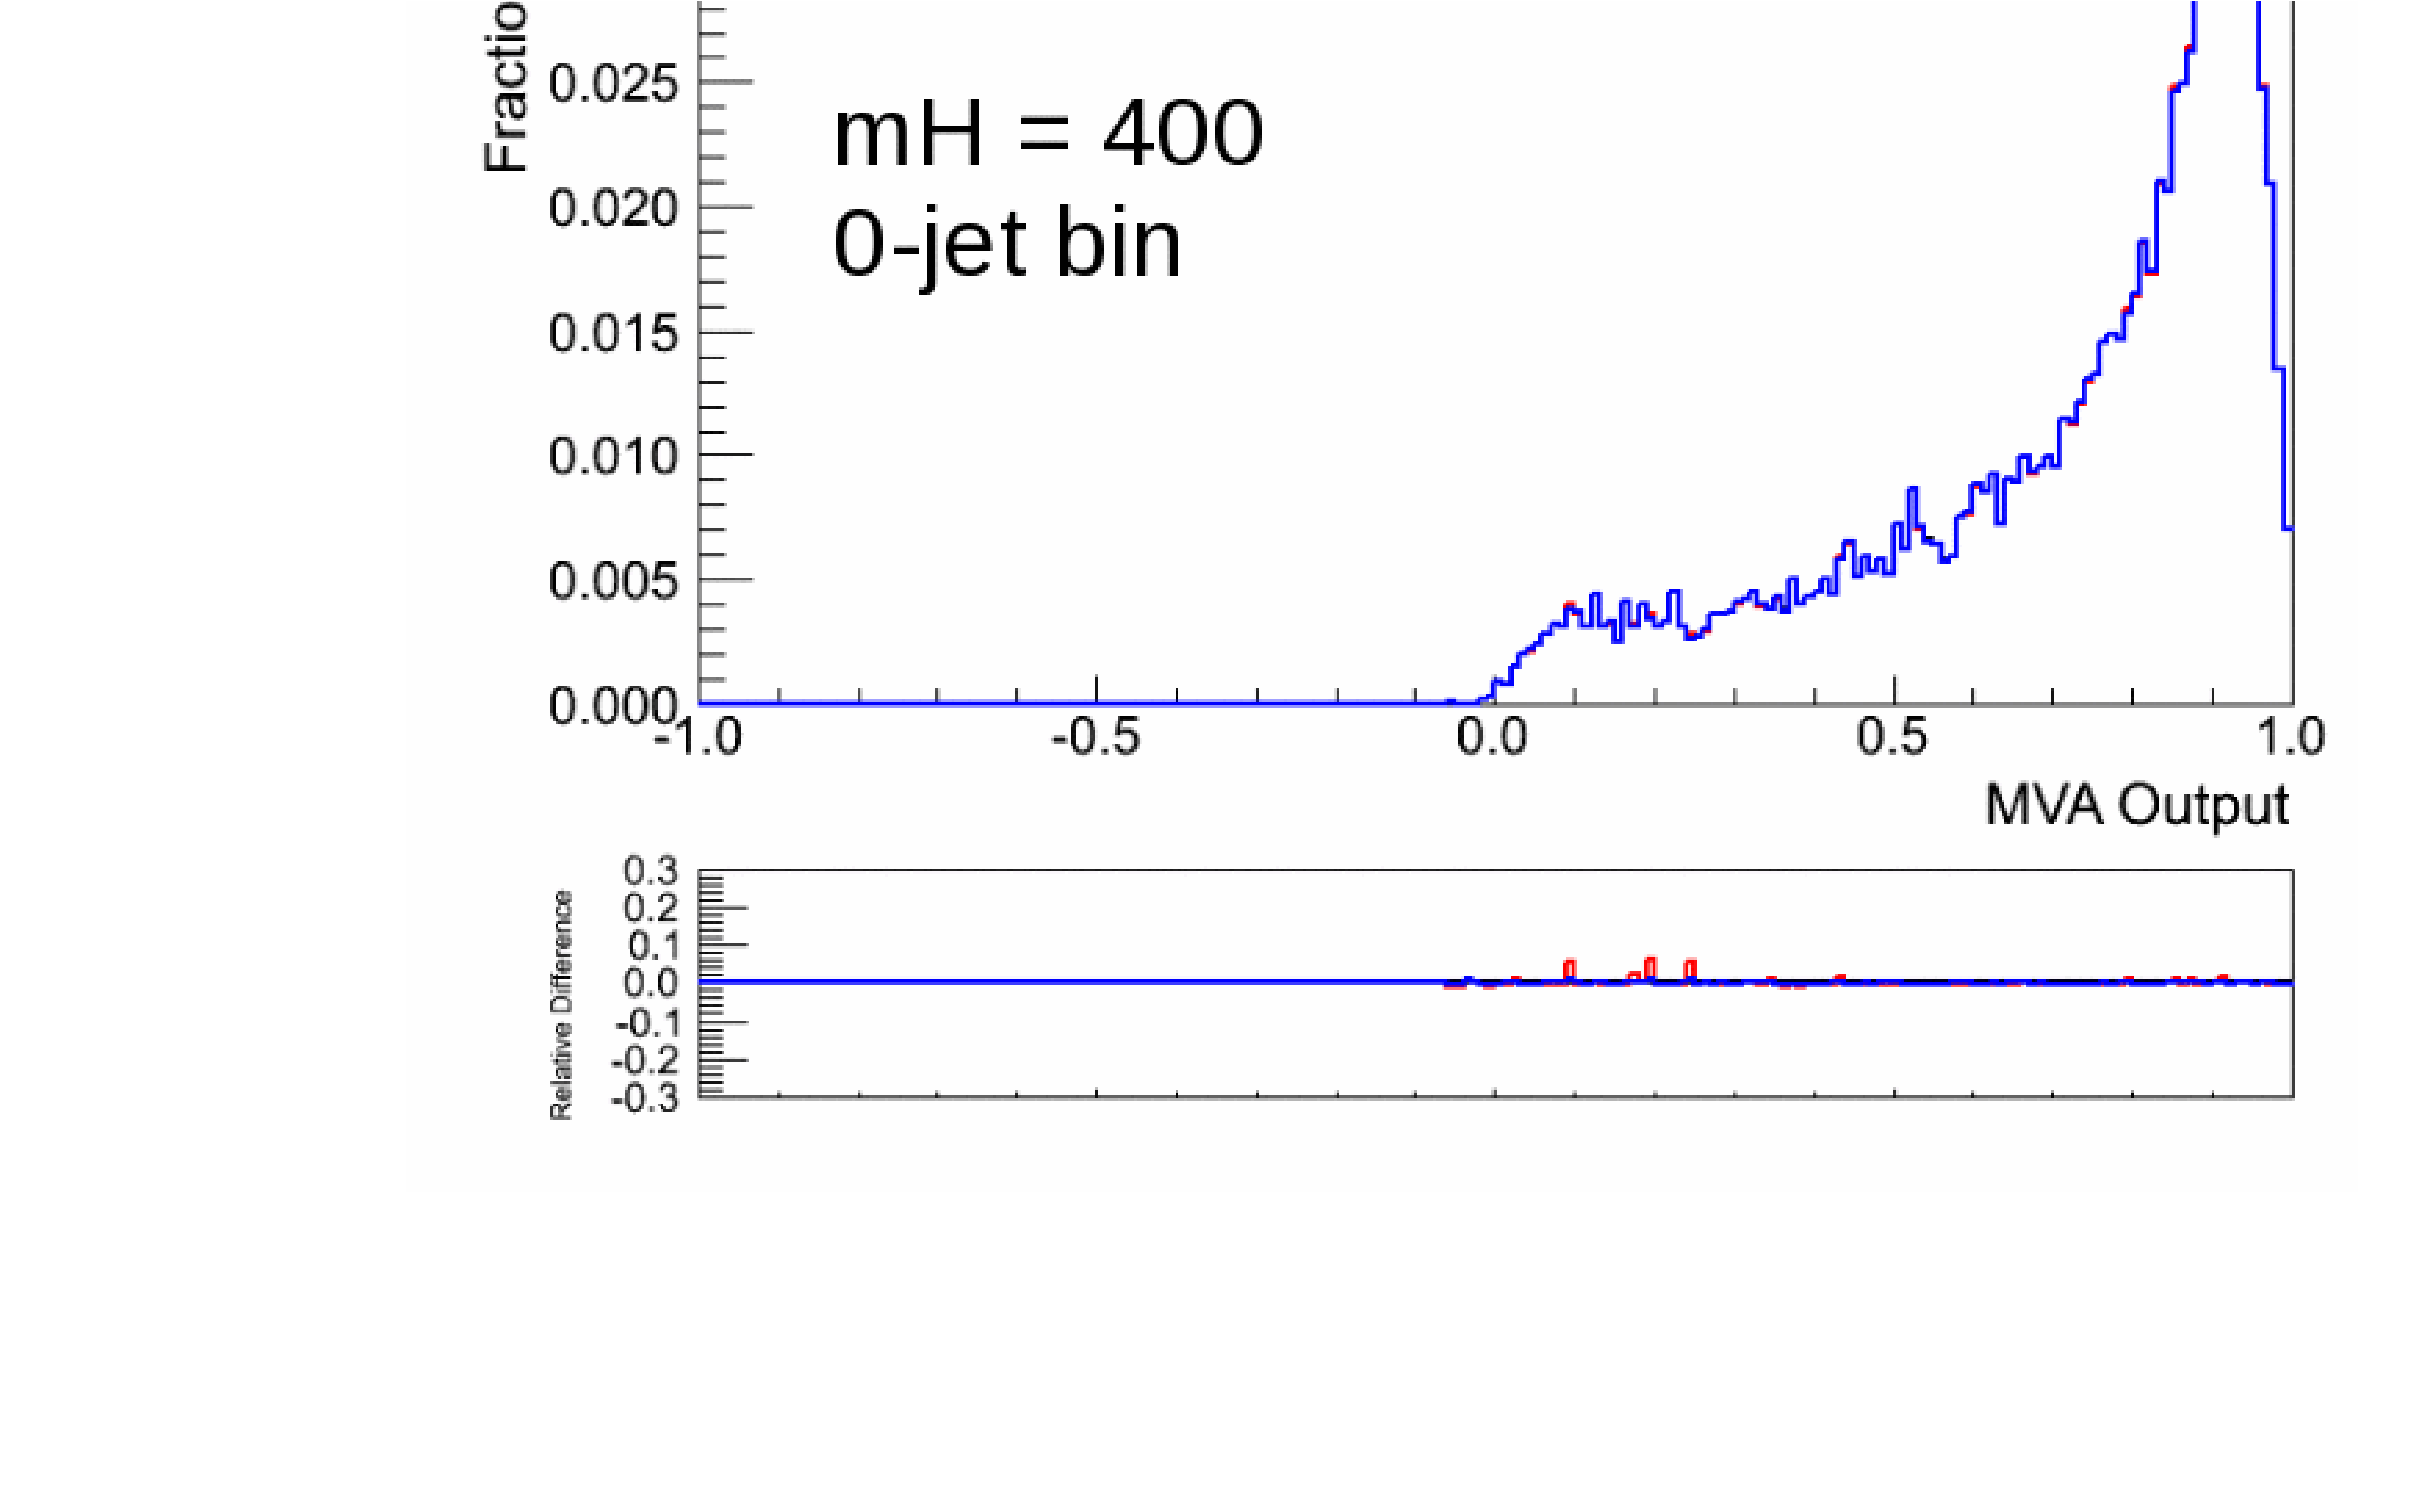
\includegraphics[width=0.49\textwidth]{figures/ShapeSystematics_HWW_MVA400_HQTScaleVariation.pdf}}
\caption{Comparison of the MVA outputs for the MVA trained on different Higgs mass hypotheses 
between the prediction of the MC reweighted to the scale varied and default $p_{T}$ spectra. 
}
\label{fig:signalshape_PtSpectrumScaleVariation_MVAOutput}
\end{center}
\end{figure}
%%%%%%%%%%%%%%%%%%%%%%%%%%%%%%%%%%%




To study the effect of higher order corrections on everything else, we produce
POWHEG Monte Carlo with the renormalization and factorization scales varied 
up and down by factors of $2$ and $1/2$, and reweight both scale varied samples
to the nominal NNLO Higgs $p_{T}$ spectrum from HQT. These predictions give 
an indication of the effect of terms beyond NLO in the perturbative expansion,
assuming that the Higgs $p_{T}$ spectrum has been fixed to the true spectrum. 
The study is performed only at generator level since the MVA input observables
are all leptonic observables which are not expected to be significantly 
affected by the simulation and reconstruction. The comparison is shown in 
Figure \ref{fig:signalshape_PtSpectrumScaleVariation_MVAOutput}
which indicates no significant differences between the scale varied and the default 
scale prediction beyond statistical uncertainties. Furthermore, the differences
between the scale varied predictions and the default scale predictions show
random behavior consistent with statistical fluctuations. 


%%%%%%%%%%%%%%%%%%%%%%%%%%%%%%%%%%%
\begin{figure}[!htbp]
\begin{center}
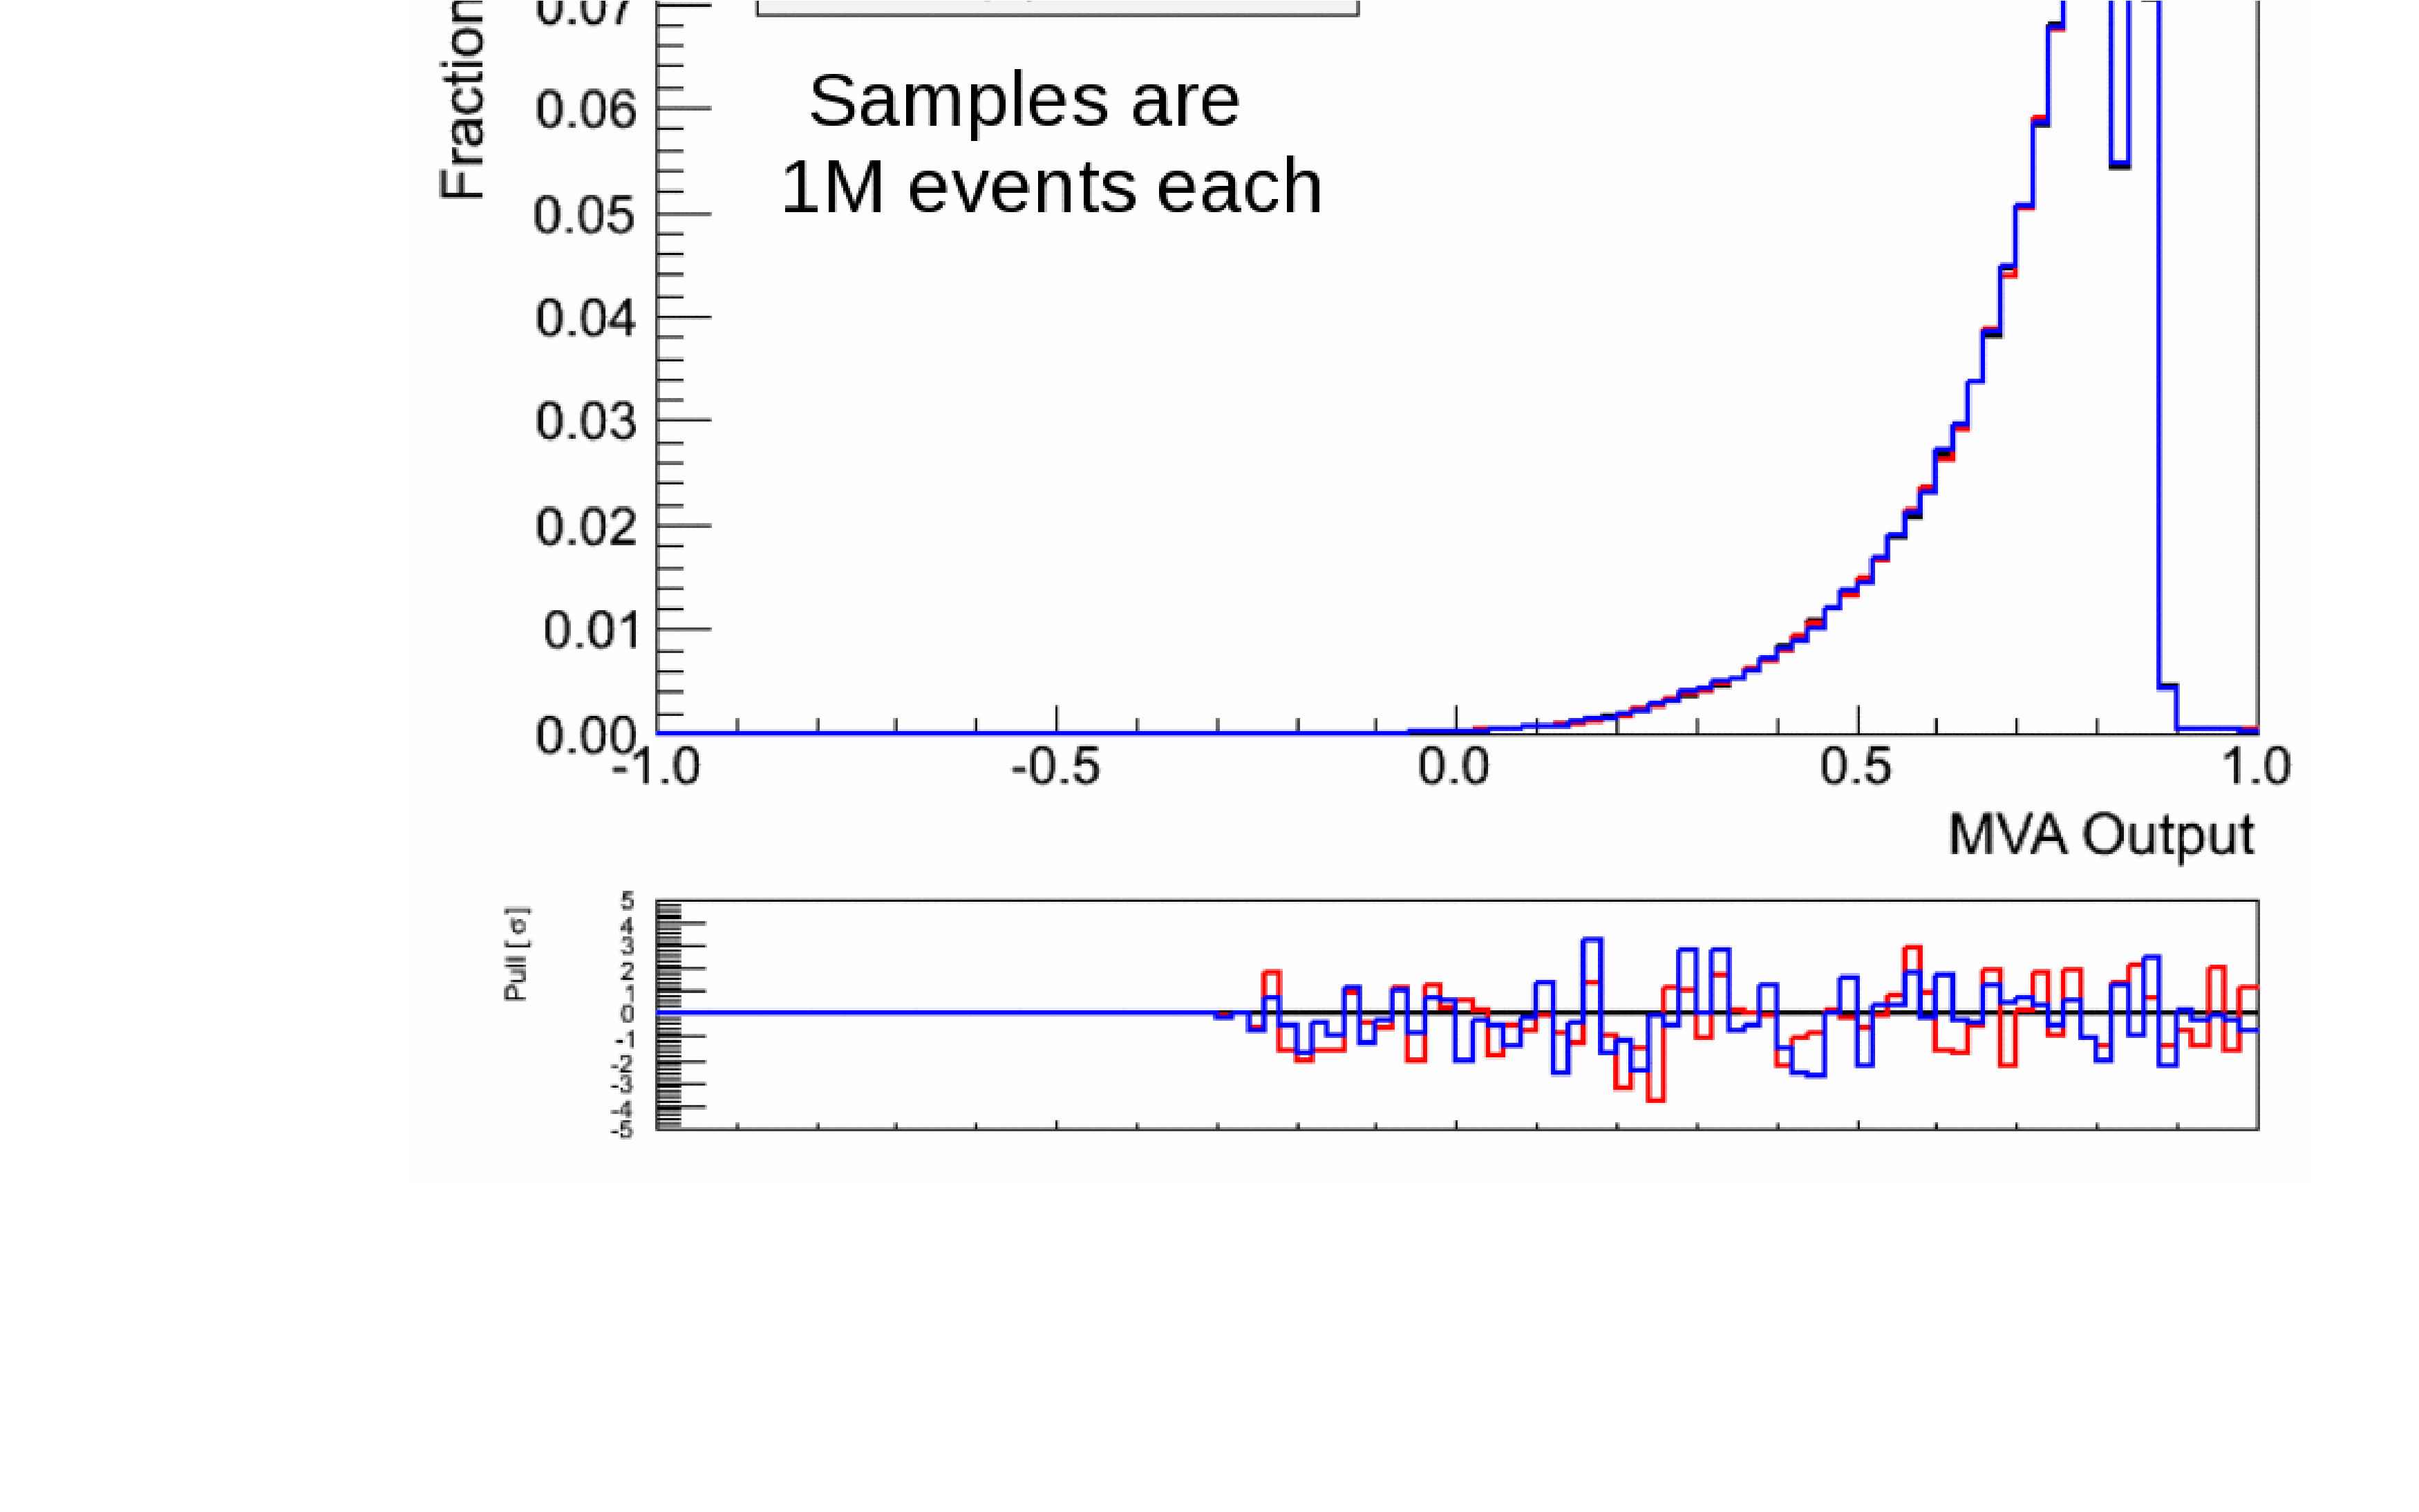
\includegraphics[width=0.49\textwidth]{figures/ShapeSystematics_HWW_MVA130_PowhegScaleVariationFixedPtSpectrum.pdf}
\caption{Comparison of the MVA output trained with the $M_{H}=130$ GeV Higgs mass hypothesis 
between the prediction of the MC reweighted to the scale varied and default $p_{T}$ spectra. 
}
\label{fig:signalshape_PtSpectrumScaleVariation_MVAOutput}
\end{center}
\end{figure}
%%%%%%%%%%%%%%%%%%%%%%%%%%%%%%%%%%%


\subsubsection{Parton Distribution Function}